%% File: elsarticle.latex
%% Purpose: Support Elsevier's `elsarticle` package through pandocomatic.
%%          To that end turn the generic `elsarticle-template.tex` into
%%          a template that can be used in conjunction with
%%          pandocomatic and scrivomatic.
%% Authors: Ian Max Andolina, Paul Brandt
%% Date   : Nov. 11, 2021
%% 
%% This file is a manual integration of:
%%      *   elsarticle-template.tex (NOT the `elsarticle-template-*.tex` 
%%          examples that appear in the elsarticle template for these are  
%%          not comprehensive enough for a full article).
%%          Sourced from https://www.latextemplates.com/template/elsarticle-academic-journal
%%      * custom.latex, a minimal portion of it to make it compatible with 
%%          pandocomatic, and removing those parts that potentially 
%%          redefine `elsarticle` definitions.
%%          Sourced from https://github.com/iandol/dotpandoc/tree/master/templates
%%
%% Backwards compatibility with both files need to be managed manually.
%%  
%% Usage notes:
%%      1 - You'd want to apply this in combination with:
%%          * pandocomatic-elsarticle.yaml, or its contents integrated
%%              in any other pandocomatic.yaml file
%%          * (optional) addstyles.sty
%%      2 - Connect <your>.md with pandocomatic's `elsevier` template
%%          * just like any other regular pandocomatic template, hence
%%          * Insert in <your>.md's yaml block:
%%            pandocomatic_:
%%              use-template:  
%%                - elsevier  
%%      2 - Run pandocomatic with <your>.md text as follows:
%%          * pandocomatic -b -c ./pandocomatic-elsarticle.yaml ./<your>.md
%%            This will generate <your>.tex, hence continue with
%%          * latexmk -interaction=nonstopmode -f -pv -time -xelatex <your>.tex
%%            This will generate <your>.pdf
%%            
%%
%% Regarding elsarticle ::
%% ---------------------------------------------
%%
%% Copyright 2007-2020 Elsevier Ltd
%% 
%% It may be distributed under the conditions of the LaTeX Project Public
%% License, either version 1.2 of this license or (at your option) any
%% later version.  The latest version of this license is in
%%    http://www.latex-project.org/lppl.txt
%% and version 1.2 or later is part of all distributions of LaTeX
%% version 1999/12/01 or later.
%%  
%%
%% Regarding dotpandoc's custom.latex ::
%% ---------------------------------------------
%% The template custom.latex is a fairly complicated piece of work 
%% (thanks to Ian Max Andolina) to produce scientific articles in a simple
%% workflow with Scrivener, pandocomatic and scrivomatic. 
%% I've taken bits and pieces from it to make the elsarticle-template
%% produce a tex document by application of a pandocomatic.yaml configuration.
%% 
%% 
%%%%%%%%%%%%%

\documentclass[sort&compress,preprint,authoryear,3p,twocolumn]{elsarticle}
%%
%% !Todo!: Resolve the conflicting `&` in `sort&compress` when parameterized as
%%         `classoption` in pandocomatic-elsarticle.yaml configuration.
%%         Currently, this parameter is added here directly as opposed to
%%         being pandocomatically configured.
%% !Todo!: Check whether one- or two-column mode has been selected, and
%%         establish the need to redefine Figures/Tables as done below.

%%%%%%%%%%%%% REQUIRED PACKAGES
%% The following packages are required for this template to remain compatible 
%% (or at least effective) with the Elsevier template.

%% Supporting colored links in citations to the References section.
\usepackage{xcolor}

%% The amssymb package provides various useful mathematical symbols
%% whereas the amsthm package provides extended theorem environments
\usepackage{amsmath,amssymb}

%% The hyperref package is required since pandocmatic inserts \hypertarget
%% around section titles and other inter-article linking.
\usepackage[]{hyperref}
% Setup hyperref to color the links, and insert authors, title and keywords
% as meta-data to the pdf document properties.
\hypersetup{
  pdftitle={Consolidating semantic interoperability in contemporary software architectural paradigms},
  pdfauthor={Paul Brandt, Eric Grandry, Marten van Sinderen, Twan
Basten},
  pdflang={en-GB},
  pdfkeywords={semantic interoperability, software
architectures, semantics, interoperability, design principles},
  colorlinks=true,
  pdfcreator={Scrivomatic, Pandoc and LaTeX}
}
%%

%%
%% Elsevier bibliography styles
%% ----------------------------
%% Elsevier requires natbib. 
\usepackage[authoryear]{natbib}
\setcitestyle{authoryear,open={(},close={)}} %Citation-related commands; modify for your convenience.
\bibliographystyle{elsarticle-harv}
%% Add extra options of natbib.sty, if any specified.

%%
%% !Todo!: Check the specifics of reference styles from elsarticle-template-*.tex
%%         as mentioned in https://support.stmdocs.in/wiki/index.php?title=Model-wise_bibliographic_style_files
%%         against the biboptions / bibliographicstyle settings from pandocomatic-elsarticle.yaml 
%% !ToDo!: Some of the bibliographicstyle settings require \usepackage{numcompress}. 
%%         Check whether this is included by this very template.
%%

%% 
%% Handle figures and tables in two-column mode
%% --------------------------------------------
%% In a two-column paper, figures and tables can become too small or overflow
%% the column width. In two-column mode we need to restore the original 
%% behaviour:
%% - For figures and tables, one needs to use the starred version * of these 
%%   environments. This floats the environment to the top/bottom of page over
%%   both columns.
%%   Source: https://tex.stackexchange.com/questions/89462/page-wide-table-in-two-column-mode
%%   Hence, redefine those environments when 'twocolumn' has been specified
    
\makeatletter
\renewenvironment{figure}{%
  \begin{figure*}
 }{% 
  \end{figure*}
 }
\makeatother
\makeatletter
\renewenvironment{table}{%
  \begin{table*}
 }{% 
  \end{table*}
 }
\makeatother
%%
%% - Longtable & xltabular do not work well with multicolumns. Therefore, 
%%   redefine these environments to enforce a single column mode before
%%   its definition, and restore the two-column mode afterwards:
\usepackage{stackengine}    % !!See Note (1) at the bottom!! 
\usepackage{xltabular}		% Include longtable with column specifier X as in tabularx
\usepackage{booktabs}		% To enhance the quality of tables in LaTeX. 
                            % Guidelines are given as to what constitutes a 
                            % good table in this context.
\usepackage{etoolbox}       % Used for the \BeforeBegin- & \AfterEndEnvironment
\BeforeBeginEnvironment{longtable}{%
    \onecolumn%
}
\AfterEndEnvironment{longtable}{%
    \twocolumn%
}
\AtBeginEnvironment{longtable}{%
    \scriptsize%
}
\BeforeBeginEnvironment{xltabular}{%
    \onecolumn%
}
\AfterEndEnvironment{xltabular}{%
    \twocolumn%
}
%%   This is not an optimal solution since it can result in pages around the
%%   longtables that are partly blank unintentionally. Other solutions to
%%   resolve this are welcome.
%%
%% !ToDo!: redefine simple tables, booktab and tabular.
%% !ToDo!: Make this part conditional on the documentclass-defined one- or
%%         two-column mode. That is, only include it when necessary.
%%


%%
%%%%%%%%%%%%% end REQUIRED PACKAGES

%%%%%%%%%%%%% OPTIONAL PACKAGES
%% The following packages are optional for this template, as
%% per the Elsevier template .

%% For including figures, graphicx.sty has been loaded in
%% elsarticle.cls. If you prefer to use the old commands
%% please give \usepackage{epsfig}

%% The lineno packages adds line numbers. Start line numbering with
%% \begin{linenumbers}, end it with \end{linenumbers}. Or switch it on
%% for the whole article with \linenumbers.
\usepackage{lineno}
\modulolinenumbers[5]

%% When you have an Orcid ID (refer to) you might want to include that
%% in your author-field as \orcidlink{<orcid>}
\usepackage{orcidlink}

\usepackage{blindtext}

%%
%% Some pandocomatic-specified options require additional packages
%%


%% Tightlist
\setlength{\emergencystretch}{3em} % prevent overfull lines
\providecommand{\tightlist}{%
  \setlength{\itemsep}{0pt}\setlength{\parskip}{0pt}}
%%

%%
%%%%%%%%%%%%% end OPTIONAL PACKAGES

%%%%%%%%%%%%% PROJECT SPECIFIC PACKAGES 
%%
%% These are managed through the `include-in-header:` parameter in the 
%% pandocomatic.yaml specification. Directly by listing the packages there, or 
%% indirectly by specifying one single file, e.g., `addstyles.sty`, that 
%% collects the required packages.
%% File   : addstyles.sty
%% Purpose: To include project specific packages without the need to insert
%%          multiplpe `header-includes:` statements in the 
%%          pandocomatic.yaml configuration file. 
%%          Although there is no functional difference between both approaches,
%%          for me this file seems to provide me with a more simple overview
%%          about which packages and their whereabouts. 
%%          Note that for this approach to work, you need to insert the name
%%          of this file in the `header-includes:` statement.     
%% Author : Paul Brandt, date Nov. 11, 2021
%%%%%%%%%%%
%
% Add your .sty files below
%
%   One can make a differentiation in where to store specific addons to your
%   LaTeX environment:
%   - Generics, i.e., re-usable ones, are maintained in folders below your TeX  
%     home directory. Use `kpsewhich -var-value=TEXMFHOME` at the command prompt 
%     to find your TeX Home. But respect the TeX Directory Structure (TDS) from
%     TeX Home downwards.
%   - Project specific stuff can be maintained in the same folder as your 
%     document for this project. 
%   No particular assumptions are made by the elsarticle templates with regard to 
%   locations of files.
%
%%%%%%%%%%%

\usepackage{mySemantics}
\usepackage{myTables}
\usepackage{myFigures}
%\usepackage{myGenerics}

\usepackage{pdflscape}      % Extends package <lscape> to add PDF support to the environment `landscape`.  
                            % Applied for table on design Principles

\usepackage{afterpage}      % Causes the commands specified in its argument to be expanded after the current 
                            % page is output. The current page will be filled up with text after \afterpage{...}.
                            % Applied for table on design Principles

\usepackage{enumitem}		% List manipulation. Customize the three basic list environments 
                            % (enumerate, itemize and description) and design your own lists, 
                            % with a〈key〉=〈value〉syntax.
                            % Applied for table on design Principles

\usepackage{gensymb}        % The gensymb package provides a number of ‘generic’ macros, 
                            % which produce the same output in text and math mode. 
                            % Used for \celsius
                            
\usepackage{cleveref}		% sourced from http://tug.ctan.org/macros/latex/contrib/cleveref/cleveref.pdf 
                            % Makes varioref clever, and reuses its work to improve its own workings. 
							% The cleveref package must be loaded after all other packages that 
                            % don’t specifically support it. Therefore, to be safe, we declare it as last 
                            % in the document's preamble.
							% Also note that all \newtheorem definitions must be placed after the 
                            % cleveref package is loaded.
\usepackage{myTheorems} 
                            
%%%%%%%%%%%
%% End of File: addstyles.sty
%%%%%%%%%%%

%%
%%%%%%%%%%%%% end PROJECT SPECIFIC PACKAGES

%%%%%%%%%%%%% DEPENDENCIES
%% When including packages by header-includes, 
%% dependencies might occur with them.
%% Resolve these dependencies below this line.
%%

%% Dependent on package{graphicx}
% Scale images - calculate the maximum dimensions first
\makeatletter
\def\maxwidth{\ifdim\Gin@nat@width>\linewidth\linewidth\else\Gin@nat@width\fi}
\def\maxheight{\ifdim\Gin@nat@height>\textheight\textheight\else\Gin@nat@height\fi}
\makeatother
% Scale images if necessary, so that they will not overflow the page
% margins by default, and it is still possible to overwrite the defaults
% using explicit options in \includegraphics[width, height, ...]{}
\setkeys{Gin}{width=\maxwidth,height=\maxheight,keepaspectratio}
% Set default figure placement to htbp
\makeatletter
\def\fps@figure{htbp}
\makeatother
%%

%%
%%%%%%%%%%%%% end DEPENDENCIES

%%%%%%%%%%%%% ADD & PARAMETERIZE elsarticle template elements

\journal{Information and Software Technology}

\begin{document}

\begin{frontmatter}

%% TITLE elements
  \title{Consolidating semantic interoperability in contemporary
software architectural paradigms\tnoteref{id1,version}}
  \tnotetext[id1]{Tables \& figures with 2-columns incorrectly placed;
will be corrected when submitting.}\tnotetext[version]{version v1.0-4}
%%

%% AUTHOR elements
  \author[1]{Paul
Brandt\fnref{0000-0002-2353-967X}\corref{corrauth}}\fntext[0000-0002-2353-967X]{ORCID: \orcidlink{0000-0002-2353-967X}0000-0002-2353-967X}\ead{paul@brandt.name}\cortext[corrauth]{Corresponding author}   \author[2]{Eric
Grandry\fnref{0000-0003-3553-8460}}\fntext[0000-0003-3553-8460]{ORCID: \orcidlink{0000-0003-3553-8460}0000-0003-3553-8460}\ead{egrandry@gmail.com}   \author[4]{Marten
van
Sinderen\fnref{0000-0001-7118-1353}}\fntext[0000-0001-7118-1353]{ORCID: \orcidlink{0000-0001-7118-1353}0000-0001-7118-1353}\ead{m.j.vansinderen@utwente.nl}   \author[1,3]{Twan
Basten\fnref{0000-0002-2274-7274}}\fntext[0000-0002-2274-7274]{ORCID: \orcidlink{0000-0002-2274-7274}0000-0002-2274-7274}\ead{a.a.basten@tue.nl}%%

%% INSTITUTE elements
\affiliation[1]{organization={Eindhoven University of Technology (TU/e),
Eindhoven, The Netherlands}} \affiliation[2]{organization={Ministry of
Mobility and Public Works, Luxembourg,
Luxembourg}} \affiliation[4]{organization={University of Twente (UT),
Enschede, The Netherlands}} \affiliation[3]{organization={ESI (TNO),
Eindhoven, The Netherlands}} 
%%

%% ABSTRACT text
\begin{abstract}
\emph{Background:} Absence of access-and-play semantic interoperability
(sIOP) is a big hurdle to contemporary IT-based business collaboration.
Current approaches towards sIOP not only impede access-and-play sIOP but
also its progress towards a standard infrastructural semantic layer.
Real-world semantics cannot exist in software and are reduced to the
reciprocity between data and data processing. Data exchange breaks that
reciprocity, failing sIOP. sIOP demands re-establishing a valid
reciprocity between the consumer's data processing and the producer's
data, without dependency on semantic standards. For access-and-play sIOP
the effort of the human-in-the-loop has to be reduced. This is a matter
of software architecture.

\emph{Objective:} The objective of our study is to identify and
formulate the fundamental demands on sIOP, to derive its supporting
architectural principles, and their integration in contemporary
architecturals.

\emph{Method:} We assess the problems and identify requirements on sIOP,
two of which demanding a human-in-the-loop. We develop design principles
for interoperability between the agents' semantics. We evaluate these
principles by designing an ISO-42010 Architecture Viewpoint and View on
sIOP.

\emph{Results:} We show that loosely coupled semantics, semantic
alignments, and accountability about the applied ontological commitment
are the cornerstones to sIOP. The supporting principles are:
responsibility for your data semantics; an explicit ontological
commitment; separating semantics from communication; aligning internal
and external semantics of exchanged data; encapsulate how agents
exchange semantics. The resulting Architecture Viewpoint and View on
sIOP, including semantic mediation, consolidates sIOP in contemporary
architectural paradigms.

\emph{Conclusions:} Our principles correct architectural shortcomings
for an access-and-play sIOP capability. Conditions supporting sIOP have
to be realised in advance of the data exchange, resulting in loosely
coupled semantics that are re-usable for different business
collaborations, even those that are not anticipated for. This paper
intents to support research into domain-independent standardised
semantic services and API's, to be adopted and embedded into the
communication infrastructure.
\end{abstract}

%%Graphical abstract
%\begin{graphicalabstract}
%\includegraphics{grabs}
%\end{graphicalabstract}

%%Research highlights
%\begin{highlights}
%\item Research highlight 1
%\item Research highlight 2
%\end{highlights}
%%

%% KEYWORDS elements
\begin{keyword}
semantic interoperability\sep software
architectures\sep semantics\sep interoperability\sep design principles
\end{keyword}
%%

\end{frontmatter}

%% Consider the use of line numbers
\linenumbers


%%%%%%%%%%%%% MAIN TEXT

\hypertarget{introduction}{%
\section{Introduction}\label{introduction}}

Never before, data were so ubiquitous, and managed access to external
data was so easy. But \emph{understanding precedes use}, and
understanding the data requires a human-in-the-loop. Therefore, semantic
interoperability (sIOP) is time-consuming and hampers agility in
business collaboration in all domains. The most disconcerting
consequences of a lack of (automated) sIOP are time-to-deliver, flat
interoperability failures, and seemingly correct but quite invalid data
comprehension that leads to faulty system behaviour. For instance,
consider the following (allegedly real) example of an interoperability
failure.

\begin{quote}
A German steel producer upgraded its industrial process robot. Since the
majority of the steel production process is dependent on time, from a
safety point of view the decision was made to not rely on their own
internal clocks but to use the German \emph{Braunschweig Funkuhr} time
radio signal as source for the exact time instead. At the end of April
1993, when Germany went on summer time, the computer clock of the steel
producer went from 1:59 AM to 3:00 AM in one minute. This resulted in a
production line allowing molten ingots to cool for one hour less than
normal. When the process controller asserted the cooling time had
expired, its actions splattered still-molten steel, damaging part of the
facility.\footnote{Source: http://catless.ncl.ac.uk/Risks/14/57\#subj1,
  accessed May 20, 2018}
\end{quote}

In this simple example a tiny difference in the meaning of \texttt{time}
between the Data Service Consumer (DSC), i.e., steel manufacturer, and
the Data Service Producer (DSP), i.e., the Braunschweig Funkuhr,
hampered interoperability to the extend of damaging the steel facility.
This tiny difference rooted in the assumption by the DSC that
\texttt{time} expressed a continuum whilst for the DSP, \texttt{time}
denoted instant clock time for the yearly season, allowing seasonal
discontinuities. Data represents a certain state of affairs (SoA) in the
domain of application (DoA), and the purpose of sIOP is to communicate
that SoA such that the DSC can act on it. Unfortunately, between the DSP
and the DSC variations may exist in terms, structures, dimensions and
other background knowledge about the exchanged data. Consequentially,
one datum might refer to two different SoAs, deceiving the DSC about its
perceived SoA, leading to conclusions that cannot be substantiated in
the DoA and, subsequently, to incorrect behaviour. In order to achieve
that DSCs can correctly \emph{use} DSPs' data, the need exists to design
and implement wrappers that restores any differences in SoAs that emerge
from the data. Many such variations exist, leading to a range of
failures in sIOP. Unfortunately, it is fundamentally impossible to
automate the production of wrappers, because we need a genuine
\emph{understanding} upfront, which computers still cannot do. When we
accept the need for a human-in-the-loop, her place in architecture
becomes a design choice. Like \citep{Kuhn2009}, and as opposed to a
philosophical or linguistic problem, we consider semantic
interoperability an engineering problem that aims at constraining
interpretations towards those that are intended, producing engineering
artefacts that can carry sIOP.

Current sIOP implementations are essentially based on the
(time-consuming) process of establishing a shared convention on the
semantics of the data that are exchanged, and require custom software
solutions and collaboration-dependent software adaptations. Indeed, such
conventions result in a pleasant semantic homogeneity, but also in huge
semantic monoliths that resolve some but far from all interoperability
problems \citep{Renner1996}. And it makes dealing with data that
originated outside the monolith impossible, unless again a time
consuming (months) semantic adoption process is applied. Moreover, these
semantic conventions consider semantic heterogeneity a bug instead of a
feature necessary to allow for different but equally valid perspectives
and to achieve semantic accuracy. Nevertheless, this conventions-based
approach towards sIOP is considered accepted folklore, even state of the
art in ICT, e.g., \citep{Otto2019}. In view of the large uptake of the
Internet, the Internet of Things (IoT), cloud computing and big data,
and in view of economical pressure to intensify enterprise
collaboration, we consider this approach insufficient. Automation is
required to resolve these issues, and we place formal semantics at its
core.

The main objective of our work is to achieve sIOP as quickly as
possible, with as minimal human effort as possible, for collaborations
that had not been foreseen and consequently could not be anticipated for
during design time of the (two or more) software agents. Semantic
heterogeneity must be allowed for, semantic scalability must become
possible. We categorise our work in terms of the Framework for
Enterprise Interoperability (FEI) \citep{Chen2017} as addressing the
\emph{conceptual} barrier, investigating the \emph{data} and
\emph{process} concerns, and applying a \emph{federated} approach.

In comparison, system scalability was a big architectural concern in the
past, requiring custom solutions as well. In response to this concern,
scalability was standardised in the form of architectural patterns, and
finally totally embedded and hidden into the infrastructure. Similarly,
sIOP can be considered the architectural concern of this decade. We
first need to provide standardised solution patterns that address sIOP
concerns before we can embed it in a technological infrastructure. Only
then we can claim that sIOP becomes transparent to the developer, and
only then we can take down the tight coupling between semantics and the
syntax of the shared data scheme. Where system scalability resulted in a
huge increase in performance-demanding applications against a fraction
of the original costs and effort, business agility will emerge once
their semantics are accessible and semantic services exist at the
infrastructural level to address them. Then sIOP becomes an
access-and-play operation that can be achieved in due time with data not
anticipated for during software design, and at any point in their life
cycle. Metaphorically speaking, we consider sIOP a bridge overarching a
semantic gap: with \emph{anchorages} (local, tangible semantics
according to \citep{Brandt2021a}) on each side of the gap, with a
\emph{spanning} (semantic alignments) resting on them to structurally
(semantically) support the interoperability bridge, and with a
\emph{roadway} (syntactic transcriptions) enabling the crossing of the
(data) traffic. Finally, architectural \emph{principles} provide the
necessary guidance to the architect for the various design decisions
that effectively result in a particular bridge over a particular
semantic gap. This has been depicted in \cref{fig:semantic-concerns}.

\begin{figure}
  \centering
  \subcaptionbox{\label{fig:concernsa}}
    [.75\textwidth]{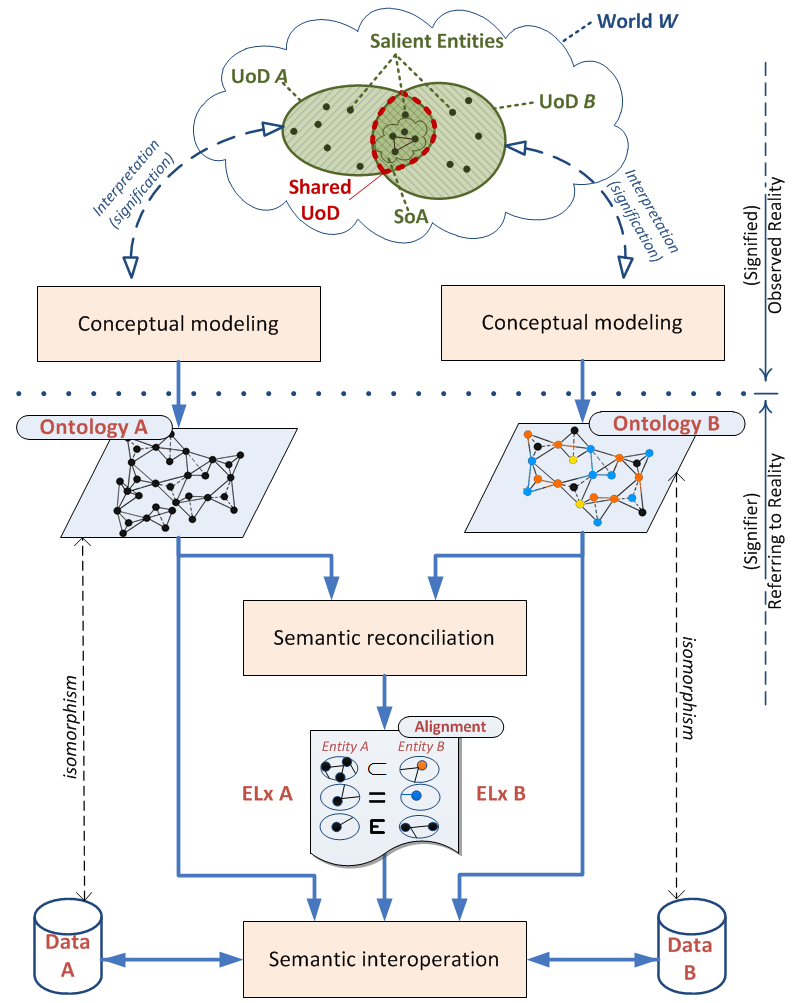
\includegraphics{src/images/3SemanticConcerns}}
  \hfill
  \subcaptionbox{\label{fig:concernsb}}
    [.15\textwidth]{\includegraphics{src/images/3ConcernsLegend}}
  \caption{Conceptual overview of the relationships in sIOP between the anchorage (conceptual modelling), its spanning (semantic reconciliation) and roadway (semantic mediation), (a), and a legend explaining the used constructs (b).}\label{fig:semantic-concerns}
\end{figure}

Our contributions to consolidating semantic interoperability in software
architectures are fivefold, represented as architectural principles and
concerns as follows:

\begin{itemize}
\tightlist
\item
  Semantic concerns (anchorage): We summarize our work in
  \citep{Brandt2021a} on how to achieve a semantic anchorage by
  abstracting semantics from a tacit software implication into a
  tangible, computational and distinct artifact. This creates the
  potential to connect to it, to make comparisons with the semantic
  artifact of the peer software agent. We then formulate the principle
  of assuming responsibility on the semantics on data, and conclude what
  preparations about semantics are required for an agent before being
  able to engage in semantic interoperability
  (\cref{anchorage-semantic-concerns});
\item
  sIOP concerns (spanning): Since computers remain incapable of true
  understanding, sIOP remains in demand of human intervention in order
  to reconcile the semantic differences between collaborating software
  agents. However, human intervention is time consuming. We establish
  principles to minimise human intervention to a level that suffices to
  achieve sIOP, viz authoring semantic alignments only
  (\cref{spanning-siop-concerns});
\item
  Mediation concerns (roadway): We determine the demands for a generic
  component that allows for communication with the peer agent in one's
  own native vocabulary only, by considering both ontological models and
  the alignment. Such approach applies the principle \emph{connectivity
  without dependency} at the semantic level. This consolidates the
  agent's potential to collaborate to any unforeseen applications
  without the need to adopt external semantic definitions, and remain
  scalable in the process (\cref{roadway-mediation-concerns});
\item
  \emph{Evaluation of semantic principles}: It is a matter of
  architectural hygiene to evaluate how the derived principles support
  and consolidate the fundamental architectural demands about loose
  coupling and separation of concerns (notably semantic and
  communication concerns). We show how the necessary characteristics of
  semantics, i.e., semantic heterogeneity, semantic evolution and
  semantic scalability, are supplied by them
  (\cref{evaluation-of-siop-principles});
\item
  ISO42010 Architecture Viewpoint: We verify the applicability of the
  above concerns and principles by formulating their architectural
  consequences as a specific ISO42010 sIOP Viewpoint that must
  consolidate their proper position in the total architecture as
  corresponding sIOP view. As ISO42010 is considered a set of best
  practises for architecture description, and therefore is used with
  architecture frameworks such as MoDAF, TOGAF, DoDAF, RM-ODP and more,
  we conclude that application of this sIOP Viewpoint to formulate the
  sIOP View can be considered to consolidate sIOP for contemporary
  architectural paradigms (\cref{iso42010-viewpoint-on-siop}).
\end{itemize}

The European Interoperability Framework
(EIF)\citep{EuropeanCommissionDGInformatics-ISA2Programme2017} and the
European Interoperability Reference Architecture (EIRA)
\citep{EuropeanCommissionDGInformatics-ISA2Programme2019} address sIOP
and recommend the separation of syntactical from semantic concerns.
Indeed, a valid recommendation that we support. In itself, though, it
renders insufficient as to the practice of how to achieve such
separation. We consider this article a principled approach to that
practice. It is our intention with this paper to open the discussion on
how to surface domain-independent and standard semantic services and
API's that can be adopted to become embedded into the communication
infrastructure.

In
\cref{anchorage-semantic-concerns,spanning-siop-concerns,roadway-mediation-concerns,evaluation-of-siop-principles}
we derive \#\# Design Principles (DPs) to consolidate the three
architectural concerns. We define them collectively as \cref{tab:dps} at
the end of the paper, following the structure in \citep{Greefhorst2011}.

\hypertarget{anchorage-semantic-concerns}{%
\section{Anchorage: Semantic
concerns}\label{anchorage-semantic-concerns}}

Since we here talk about \emph{semantic} interoperability, we first need
to establish what is meant with semantics in software. We then defend
the need for semantic heterogeneity and finally

\hypertarget{semantics-in-software}{%
\subsection{Semantics in software}\label{semantics-in-software}}

With semantics, we refer to real world semantics (RWS) and we summarise
our position towards semantics in software from \citep{Brandt2021a} as
follows:

\begin{itemize}
\tightlist
\item
  Since software is incapable of genuine understanding, real world
  semantics cannot exist in software. Nevertheless, the software agent
  acts as transport medium for RWS between users and must do so without
  compromising the transported cargo, viz RWS.
\item
  Based on \citep{Grice:1991BT}, we discern \emph{semantic meaning},
  i.e., what is said and carried by data, and \emph{pragmatic meaning},
  i.e., to connect with our frame of reference and its context of use,
  implementing comprehension as an inference process from the semantic
  meaning.
\item
  We consider \emph{data} the carrier for semantic meaning, and their
  \emph{data processing} carrier for pragmatic meaning.
\item
  The nature of software dictates that data and their data processing
  are always intimately connected. We consider the \emph{reciprocity}
  between data (semantic meaning) and their processing (pragmatic
  meaning) the carrier of RWS.
\item
  Any incoherent reciprocity, i.e., inconsistencies between data and
  their processing code, equates to unfaithfulness to reality, viz
  semantics that are considered invalid by the current SoA in the
  application domain.
\item
  The central disposition of reciprocity in software semantics emerges
  as an \emph{Atomic Semantic Monolith} (ASM), established with the
  explicit purpose to guarantee the coherence between the data (semantic
  meaning) and their processing code (pragmatic meaning) required to
  achieve data comprehension.
\item
  The Domain Model (DM), composed as the combination of the Semantic
  model (representing all semantic meanings) with the Pragmatic Model
  (representing all pragmatic meanings), provides the software agent
  with the level of comprehension necessary to decide upon its behaviour
  (to achieve the agent's objectives) under the current state of
  affairs.
\item
  In the active, processing, part of an agent we thus separate
  comprehension, specified by the DM, from behaviour, specified by the
  System Model (SM). We consider the SM semantically grounded in the DM
  if all terms that are used by the SM to refer to the DoA, get their
  comprehension from the DM.
\end{itemize}

\hypertarget{semantic-heterogeneity}{%
\subsection{Semantic heterogeneity}\label{semantic-heterogeneity}}

``The successful standardisation of protocols made us believe that we
should also \emph{standardise meaning} on the Web. This is a fundamental
\emph{misconception}.'' \citep{Janowicz:2013ui}. This believe can be
witnessed by the many initiatives taken by standards developing
organisations (SDO) to develop a myriad on data standards, from e.g.,
\emph{Tradelens} in Transport \& Logistics domain and
\emph{International Financial Reporting Standards} in Finance \&
Accounting to, e.g., \emph{ICEN/EN 13606}, \emph{SO/TC 215}, and
\emph{ISO/HL7 21731} in the Electronic Health Records domain and the
\emph{smartM2M} standard by the IoT European Platform Initiative
\citep{ETSI2019}, to name a few. This current viewpoint on semantics
defies semantic heterogeneity and enforces semantic homogeneity: one
single agreed domain convention on how the syntactic representation and
structure of the data or messages shall be semantically interpreted.
Indeed, semantics are a particular representation of some part of the
world, viewed from a particular perspective of use, however, we don't
acknowledge that the \emph{particular} representation and
\emph{particular} perspective that the data standard enforces is
universally shared by the domain users. And equally important, any
particular perspective is just one out of many equally legitimate ones
that our software are deemed to consider over the software's lifecycle.
Some examples are given in \cref{tab:perspectives}.

\begin{longtable}[]{@{}
  >{\raggedright\arraybackslash}p{(\columnwidth - 10\tabcolsep) * \real{0.2500}}
  >{\raggedright\arraybackslash}p{(\columnwidth - 10\tabcolsep) * \real{0.1724}}
  >{\raggedright\arraybackslash}p{(\columnwidth - 10\tabcolsep) * \real{0.1810}}
  >{\raggedright\arraybackslash}p{(\columnwidth - 10\tabcolsep) * \real{0.1810}}
  >{\centering\arraybackslash}p{(\columnwidth - 10\tabcolsep) * \real{0.0517}}
  >{\raggedright\arraybackslash}p{(\columnwidth - 10\tabcolsep) * \real{0.1638}}@{}}
\caption{Semantics follow many alternative but equally legitimate points
of view on reality, implying that no single one true abstraction exists.
Hence, semantic heterogeneity is a feature that should be preserved, as
opposed to a bug that should be sought to correct.
\label{tab:perspectives}}\tabularnewline
\toprule
\begin{minipage}[b]{\linewidth}\raggedright
Reality to refer to
\end{minipage} & \begin{minipage}[b]{\linewidth}\raggedright
Perspective \#1
\end{minipage} & \begin{minipage}[b]{\linewidth}\raggedright
Perspective \#2
\end{minipage} & \begin{minipage}[b]{\linewidth}\raggedright
Perspective \#3
\end{minipage} & \begin{minipage}[b]{\linewidth}\centering
\ldots{}
\end{minipage} & \begin{minipage}[b]{\linewidth}\raggedright
Perspective \#n
\end{minipage} \\
\midrule
\endfirsthead
\toprule
\begin{minipage}[b]{\linewidth}\raggedright
Reality to refer to
\end{minipage} & \begin{minipage}[b]{\linewidth}\raggedright
Perspective \#1
\end{minipage} & \begin{minipage}[b]{\linewidth}\raggedright
Perspective \#2
\end{minipage} & \begin{minipage}[b]{\linewidth}\raggedright
Perspective \#3
\end{minipage} & \begin{minipage}[b]{\linewidth}\centering
\ldots{}
\end{minipage} & \begin{minipage}[b]{\linewidth}\raggedright
Perspective \#n
\end{minipage} \\
\midrule
\endhead
Waves are & \emph{objects} that I can point at & \emph{forces} exerted
on dikes, walls or oil rigs & an \emph{accumulation} of other waves &
\ldots{} & a \emph{relation} between water, current, wind and the
seabed \\
\(\;\) & & & & & \\
How many terrorist attacks can be counted on 9/11? & 1, the number of
involved terrorist groups & 2, the number of collapsed towers & 4, the
number of involved aircraft & \ldots{} & 2996, the number of
casualties\footnote{as mentioned by Wikipedia,
  https://en.wikipedia.org/wiki/Casualties\_of\_the\_September\_11\_attacks,
  accessed Dec 13, 2018} \\
\bottomrule
\end{longtable}

We consider semantic homogeneity only a solution for small scale
domains, i.e., with a handfull of actors, and for a short lifespan. For
larger domains and/or longer lifespans, it is not only an illusion, but
striving for homogeneity brings about several important disadvantages:
(i) implementation of semantic standards involves considerable expenses,
and tends to solidify in software by implicit operations on data that
are expensive to change, slowly setting the standard in stone; (ii)
since semantic standards fix representation, semantics become conflated
with syntax, making the semantic standard susceptible to variations in
syntax that occur with increasing stakeholders or with contextual
evolution over time; (iii) conflating semantics and syntax create
dependencies of the semantic standard with the architectural paradigm,
its particular implementation or applied technology; (iv) the previous
three issues bring about a high impedance for the standard to change and
to evolve; and they create a significant barrier (v) for new business
opportunities, (vi) obstructing business agility, and (vii) disable a
level playing field for newcomers that have to invest hugely to adopt
the standard and reap its benefits. Essentially, it is sheer impossible
to create for each particular domain, or part thereof, a semantic
standard; even in the highly protocolised health domain that already
addressed semantics in 1987 \citep{Spronk2014}, adoption of its
standards remains slow and cumbersome {[}REF{]}. This becomes all the
more clear when comparing with the successful adoption of 2G GSM
telecommunication standard, including its evolution to 2.5G, 3G, 3.5G,
4G and 5G standards during roughly the same era. Finally, these issues
only worsen when extending sIOP to support inter-domain
interoperability.

We formulate the first (semantic) concern on sIOP:

\begin{itemize}
\tightlist
\item
  \emph{concern 1}: Acknowledge semantic heterogeneity as point of
  departure when establishing sIOP.
\end{itemize}

This immediately leads to the definition of \cref{dp:shf} in
\cref{tab:dps} to its effect. We do not imply with this principle to
abandon each and every use of semantic homogeneity. We consider shared
semantic homogeneity a useful element to achieve sIOP. However, the
principle encourages to not \emph{assume} semantic homogeneity a
necessary condition nor a point of departure when engineering sIOP.

\hypertarget{the-four-maxims-of-communication}{%
\subsection{The four maxims of
communication}\label{the-four-maxims-of-communication}}

It is clear that sIOP encompasses a communication between at least two
agents. Communication between human agents brings about a natural
responsibility for both, described by \citep{Grice:1991BT} in four
\emph{maxims} as the particular purpose of communication. We consider
these maxims as relevant for software agents as for human agents, viz to
serve:

\begin{enumerate}
\def\labelenumi{\arabic{enumi}.}
\tightlist
\item
  Quantity: Make your contributions as informative as is required (for
  the current purpose of the exchange), and not more than is required;
\item
  Quality: Do not say what you believe to be false, or for which you
  lack evidence;
\item
  Relation: Be relevant (to the immediate needs);
\item
  Manner: Avoid obscurity of expression, ambiguity, and be brief and
  orderly.
\end{enumerate}

Based on this perspective on software semantics, we formulate the second
(semantic) concern on sIOP and its elaboration in two subconcerns:

\begin{itemize}
\tightlist
\item
  \emph{concern 2}: It is a natural responsibility for software agents
  that engage in collaboration to adhere to Grice's four maxims

  \begin{itemize}
  \tightlist
  \item
    \emph{concern 2.1}: explicitly representing the semantics of their
    data in their DM (maxims 1 and 4);
  \item
    \emph{concern 2.2}: ensuring the validity and accuracy of one's data
    and related semantics (maxim 2).
  \end{itemize}
\end{itemize}

Maxim 3 relates to the purpose that the software agent is to achieve.
Since we assume that any received data refers to the (possibly changed)
SoA in the shared DoA, hence, relevance to the software agent can be
considered a matter of fact. Maxim 3 also relates to the software
agents' interoperation itself as opposed to the semantic concern of one
of them; this will be addressed in \cref{spanning-siop-concerns}.

Concern 2.1 immediately leads to the definition of \cref{dp:rfsm} in
\cref{tab:dps} to its effect. We elaborate on concern 2.2 as follows. In
\citep{Brandt2021a} we have identified that each modelling language
carries its own ontological commitment, i.e., the differences that the
language constructs characterise represent a commitment to what the
language commits to about what exists in reality. The choice of
modelling language, therefore, has major impact on the (accuracy of the)
semantics that are modelled. This semantic concern is therefore
influenced by the ontological commitment. We introduce a definition on
\emph{semantic compatibility} to its end. Merriam-Webster defines
\emph{compatibility} as ``being a computer designed to operate in the
same manner and use the same software as another computer''\footnote{Merriam-Webster,
  https://www.merriam-webster.com/dictionary/compatibility, accessed Jan
  2021}. This leads to the following definition:

\begin{mmdef}[semantic compatibility]\label{def:semantic-compatibility}
Semantic compatibility reflects that a software agent is designed to interpretate data according to the same semantic principles, distinctions and rules, viz use the same ontological commitment, as another software agent. 
\end{mmdef}

We formulate \cref{dp:scp} in order to defend that it should be possible
to investigate whether semantic compatibility exists before assessing
the validity and applicability of the semantic meaning that is carried
by data.

Where it is the objective of semantics to maximise and maintain the
coherence of the ASM, it is the objective of sIOP to address this
monolithic nature of the ASM, as we do in the next section.

\hypertarget{spanning-siop-concerns}{%
\section{Spanning: sIOP concerns}\label{spanning-siop-concerns}}

The FAIR data principles (Findability, Accessibility, Interoperability
and Reuse)\footnote{FAIR Principles,
  https://www.go-fair.org/fair-principles/, accessed Jan 2021} describe
``machine-actionable states'' that ``\emph{enable the agent (\ldots) to
have the capacity, when faced with a digital object never encountered
before, to: a) identify the type of object (with respect to both
structure and intent), b) determine if it is useful within the context
of the agent's current task (\ldots), c) determine if it is usable, with
respect to license, consent, or other accessibility or use constraints,
and d) take appropriate action, in much the same manner that a human
would. (\ldots) {[}The{]} ultimate machine-actionability occurs when a
machine can make a useful decision regarding data that it has not
encountered before.}'' \citep{Wilkinson2016}. These states resonate with
our view on sIOP, although we consider state (c) out of scope for sIOP.
We consider state (d) not a matter of sIOP per sé but one that addresses
the design of a single software agent, which has already been addressed
in \citep[DP 2]{Brandt2021a} where we have made a clear separation
between semantic comprehension at the one hand, and the behaviour of the
software agent that is based on that comprehension at the other. Having
scoped the FAIR principles in this way, the main concern for sIOP, then,
is to identify the type of object that the exchanged data belongs to,
position its values in the proper value space, and derive the
conclusions based upon which the DSC will act.

From this, we establish the sIOP concerns in the first subsection, and
address them in
\cref{positioning-the-human-in-the-loop;siop-engineering-principles}.

\hypertarget{re-establish-semantic-coherence}{%
\subsection{Re-establish semantic
coherence}\label{re-establish-semantic-coherence}}

Semantic interoperability is about at least two software agents, in
their roles as DSP and DSC, that share a particular DoA and exchange
data that represent a certain SoA in their shared reality. Subsequent to
the exchange, the data will be processed by the receiving DSC. It stands
to reason that understanding the data precedes their faithful use, which
is supported by FAIR's machine-actionable states. This also resonates
with Maxim 3, relevancy of the communication; it addresses the objective
of the DSC through its application to her pragmatic meaning.

We assume the presence of domain models, one for each collaborating
software agent, anchoring the semantics of the collaboration. Since data
represent semantic meaning only, then by exchanging data, the
represented semantic meaning are necessarily separated from the DSP's
ASM they belong to. (Why it is useless to exchange the complete ASM in
order to establish sIOP, is left as an exercises to the reader
\footnote{\rotatebox{180}{\parbox{0.44\textwidth}{Communicating the semantic monolith, although possible, results in a too narrow solution towards sIOP because this would require each agent to have an exactly equal perspective on reality. Although possible, this will rarely be the case.}}}.)
Consequently, it loses its coherence with its original pragmatic
meaning. The DSC must establish a new reciprocity with its own pragmatic
meaning. Unless it can be guaranteed that the new reciprocity is as
coherent as necessary for a faithful comprehension, it's impossible to
establish sIOP without emergence of phantom semantics. We repeat our
definition on semantic coherence from \citep{Brandt2021a}:

\begin{mmdef}[Semantic coherence]\label{def:semantic-coherence}
Semantic coherence builds on the consistency with which the [semantic and pragmatic meanings] (...) commit to the same distinctions in their shared reality, and only require each other's knowledge in executing their reciprocity. 
\end{mmdef}

We indicated in \cref(the-four-maxims-of-communication) that Maxim 3,
\emph{be relevant (to the immediate needs)}, also relates to the
interoperation between the agents. Apart from its place in the
communication protocol (what we do not address here), we consider the
ability to establish the relevancy to the immediate needs a prerequisite
for sIOP, including its communication protocol. Again, this refers to
the purpose that the software agent, now the DSC, is to achieve and,
therefore, relates directly to the above semantic coherence.

Our third concern about sIOP is founded on FAIR's machine-actionable
stance and Maxim 3 as:

\begin{itemize}
\tightlist
\item
  \emph{concern 3}: subsequent to data exchange, the DSC must have the
  capability to re-establish semantic coherence between the external
  (DSP's) semantic meaning and its own internal pragmatic meaning, and
  assure that the reciprocity between DSP's data and DSC's data
  processing code remains truthful to the state of affairs in reality.
\end{itemize}

We note that concern 3:

\begin{enumerate}
\def\labelenumi{\arabic{enumi}.}
\tightlist
\item
  applies to both the data it receives from the DSP as to the data that
  the DSC can infer from them. Although this is implied by the
  principles that lead to the emergence of what we've called the Atomic
  Semantic Monolith in \citep{Brandt2021a}, we make this consequence
  explicit here;
\item
  is to be considered recurrently when sIOP is to allow for semantic
  evolution. This demands for continued maintainability and governance
  of sIOP;
\end{enumerate}

Although they share the same semantic meaning, the resulting semantic
monolith of the DSC must be allowed to differ from the DSP's semantic
monolith. For example, by exchanging a heartbeat both agents share the
semantic meaning about the number of beats per second, however the
pragmatic meaning can vary between an indication of health for an
health-care application and an indication of performance potential in a
sports application, with different demands on semantic meaning, e.g.,
resolution and accuracy. Semantic heterogeneity thus, brings about the
fourth concern about sIOP, i.e., that of scalability, since semantics
won't be centrally coordinated anymore resulting in semantic definitions
that are distributed all over the place (see \cref{dp:shf}).

\begin{mmdef}[Semantic scalability]\label{def:semantic-scalability}
Semantic scalability is the capability of a system of collaborating agents to adopt and/or consolidate, with acceptable lead time and costs, increasing perspectives on -or more complex semantic heterogeneity about- their shared reality without compromising sIOP between any interacting software agents. 
\end{mmdef}

We elaborate the scalability concern in two subconcerns:

\begin{itemize}
\tightlist
\item
  \emph{concern 4.1}: sIOP requires to allow for scalable semantics.
\item
  \emph{concern 4.2}: Pursuing sIOP between heterogeneous semantics
  requires that the ASM's from both agents remain independent from each
  other, viz establishing a semantical loose coupling between both
  agents.
\end{itemize}

We identify two complementary aspects from these concerns. One revolves
around the human task and, therefore, impede the ``access-and-play''
business demand. Another refers to engineering challenges about
mechanisation and efficiency. We address the human tasks concerns in the
next section, and then investigate the engineering challenges in its
subsequent section.

\hypertarget{positioning-the-human-in-the-loop}{%
\subsection{Positioning the
human-in-the-loop}\label{positioning-the-human-in-the-loop}}

Access-and-play sIOP is the ultimate objective: ideally, sIOP between
agents can be achieved instantaneously, particularly for unforeseen
collaborations and preferably mechanically, i.e., without human
intervention. Despite the latter's conflict with our position, viz that
computers lack the capability for genuine comprehension, its business
benefits are too significant not to continue to strive for. Still, the
purpose of comprehension is to reconcile semantic differences, which
remains a distinct concern. Its resolution will depend on the position
that is taken on comprehension, and from our position its resolution
requires a human-in-the-loop for understanding and resolving the
semantic differences between the interoperating agents. The
architectural issue then becomes where to position the dependency on the
human for concern 3: semantic reconciliation. The three possible
approaches for the DSC about this task are:

\begin{enumerate}
\def\labelenumi{\roman{enumi}.}
\tightlist
\item
  To depend on semantic meaning that is solidified in representation: a
  semantic standard. The human task is then to create the standard and
  align the semantic meaning of both the DSP and DSC to the semantic
  standard;
\item
  To modify the DSC's own pragmatic meaning such that it can operate in
  a valid way on the external (DSP's) semantic meaning; or
\item
  To modify the external (DSP's) semantic meaning such that it can be
  operated on by the DSC's existing pragmatic meaning in a manner
  faithful to the current state of affairs.
\end{enumerate}

We already indicated that the first approach defies semantic
heterogeneity and introduces many disadvantages. The second approach
allows external definitions to influence internal workings. This clearly
breaks one of the fundamental principles of software engineering,
\emph{low coupling, high cohesion} \citep[e.g.,][]{Hitz1995}, which
complicates concern 4.2, impedes 4.1 and should be considered untenable
for concern 3, particularly its second Note. Contrarily, the last
approach respects this fundamental principle and does not impair any of
the other concerns. It \emph{does} assume the semantic variations to be
resolvable and representable. Still, re-establishing reciprocity now
becomes a threefold task: First, to reconcile all semantic differences
between the representations of the Domain of Interpretation that is
shared by the DSP and DSC. Second, to represent that reconciliation in a
formal language that allows for mechanical transcription of the data
representation provided by the DSP to the data representation applied by
the DSC, without inducing phantom semantics. Third, to make the former
two tasks as efficient as possible.

\textbf{Semantic reconciliation}

A prerequisite to this task is that DSP's ASM refers to a SoA that can
be addressed by DSC's ASM when processing the received data. For this to
hold, we first require that the quality of the DSC and the DSP is such
that their internal semantic meaning is in coherence with their internal
pragmatic meaning, i.e., that their concerning ASMs are faithful to
reality over the complete value range of their internal semantic
meaning. Provided that the principles of \citep{Brandt2021a} have been
followed, this requirement is met. Now assume that the semantic meaning
that the DSP is to exchange, is equivalent to some semantic meaning that
is in scope with the DSC software agent. By virtue of the coherence that
is in place with the DSC software agent, the reciprocity between the
external semantic meaning with the internal pragmatic meaning can be
guaranteed to be re-established since there is no semantic difference
with the internal semantic meaning. The only difference to overcome is
the differences in representation between the external and internal
semantics meanings.

\textbf{Representing alignments}

\textbf{Efficiency}

\begin{center}\rule{0.5\linewidth}{0.5pt}\end{center}

++++++++++++

tbv tweede deel van de taak (human efficiency) This can be achieved by a
transcription process that can be generic and only requires a
specification of how the external semantic meaning relates to what
internal semantic meaning. This specification is known as a semantic
alignment.

Unfortunately, we cannot assume full equivalence between the semantic
meanings of the DSP and the DSC. Indeed, many variations in semantic
meaning can exist. However, there is no reason to assume the existence
of semantic variations for which no alignments can be specified. We
reflect this with \cref{dp:alignment}.

A \emph{correspondence} specifies as accurately as possible the semantic
differences that exists between a pair of related concepts, i.e., it
aligns between the semantic meanings of interoperating agents. By
exhaustively addressing all semantic differences that exist between both
agents, the set of correspondences collectively specify the
\emph{alignment} that holds between two agents. The purpose of the
alignment is to establish how the truth of expressions that are
formulated in terms of the DSP, can be established by using formulations
in terms of the DSC, and to capture this as a semantic
\emph{correspondence}. To that end we differentiate between two
categories of semantic differences:

\begin{enumerate}
\def\labelenumi{\arabic{enumi}.}
\tightlist
\item
  \emph{Ontological differences}: variations that root in philosophical
  principles\footnote{The formal tools of ontological analysis include
    theories of Essence and Identity; Parts (Mereology); Unity and
    Plurality; Dependence; Composition and Constitution; Properties and
    Qualities; and Space and Time.} and can be specified as logical
  relation between (constructions of) concepts from both ontologies,
  e.g., naming conventions, structural variations, or Class-vs-Property
  differences;
\item
  \emph{Value differences}: variations in conventions on how to
  represent values with or without magnitudes, e.g., differences in
  value scales, units of measure or nominal properties.
\end{enumerate}

The language used to specify correspondences must be expressive enough
to identify the atomic elements of the ontologies, to combine them into
logical combinations as well as to formulate the relationship that holds
between them. In \citep{Euzenat2007}, an investigation has been reported
towards the requirements for such an alignment language, resulting in
EDOAL \citep{Scharffe2011}. By application of \emph{conceptual
connectors} the architecture gains the capability to address a specific
compound of individuals in either the source or target ontology that
relate to the semantic difference at hand, resolving the above
ontological differences. Similarly, with the application of \emph{value
functions}, the architecture gains the capability to overcome the above
value differences by specifying transformations between conventions on
value representations, nominal properties or unit conversions.

Current sIOP practises already require humans-in-the-loop to reconcile
the semantic differences that occur. Often, the subject of
reconciliation is the differences in data schemata, and the result of
the reconciliation is laid down as a canonical data model. By applying
semantic reconciliation on the conceptual level, the dependency on the
(data) syntax, and vice-versa, is minimised. Moreover, by representing
the result of the reconciliation as an alignment (between ontologies) as
opposed to a canonical semantic model (core ontology), the influence of
the peer agent's semantics on one's own semantics is minimised as well.
An alignment, thus, functions as an interface that enforces loosely
coupled semantics by enabling semantic transparency between
communicating peers. Reducing the human-in-the-loop to author an
alignment only, (i) accelerates the deployment of sIOP by removing all
human effort that is concerned with implementation activities, and (ii)
decouples the sIOP scope to bilateral alignments only. This process has
been depicted in \cref{fig:dt-reconciliation}.

\begin{figure}
\hypertarget{fig:dt-reconciliation}{%
\centering
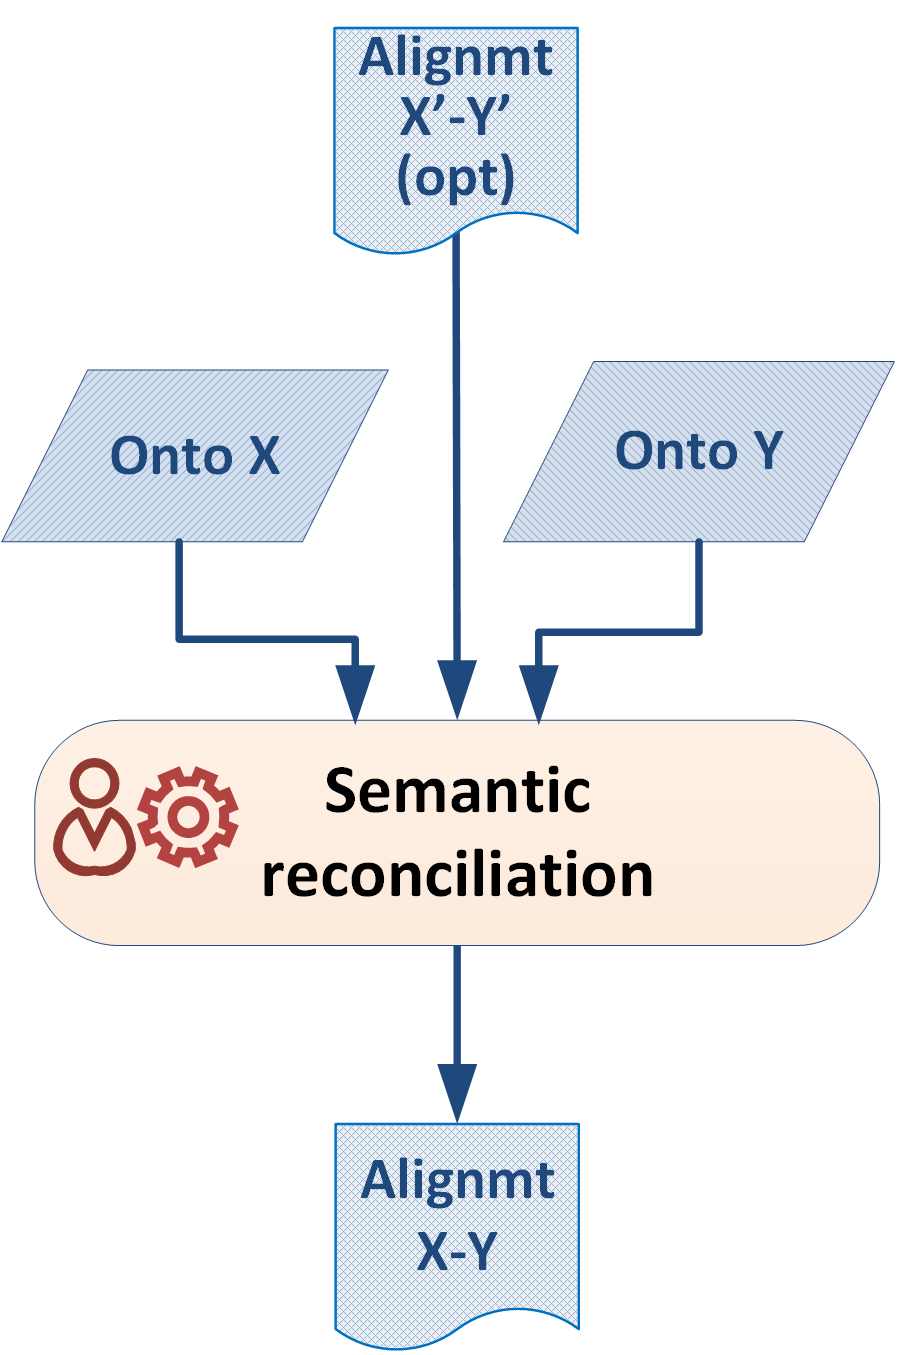
\includegraphics[width=0.25\textwidth,height=\textheight]{src/images/DesignTimeReconciliation.png}
\caption{Semantic reconciliation results in an alignment between the
semantic representations of two ontologies. We defend that semantic
reconciliation is a computer-aided but ultimately human-authored
task.}\label{fig:dt-reconciliation}
}
\end{figure}

\hypertarget{siop-engineering-principles}{%
\subsection{sIOP engineering
principles}\label{siop-engineering-principles}}

Address concerns 3.2, 4.1 and 4.2

\begin{itemize}
\item
  \emph{concern 3}: subsequent to data exchange, the DSC must have the
  capability to re-establish coherence between the external (DSP's)
  semantic meaning and its own internal pragmatic meaning, and assure
  that the reciprocity between DSP's data and DSC's code remains
  truthful to the state of affairs in reality.
\item
  \emph{concern 3.3}: Access-and-play sIOP is the ultimate objective:
  ideally, sIOP between agents can be achieved instantaneously, also for
  unforeseen collaborations. Despite its conflict with our position that
  software is incapable of genuine understanding, turning a
  human-in-the-loop a necessary condition for sIOP, its business
  benefits are too significant not to continue to strive for it;
\item
  \emph{concern 4.1} : sIOP requires to allow for scalable semantics.
\item
  \emph{concern 4.2}: Pursuing sIOP involves to ensure that the ASM's
  from both agents remain independent from each other, viz establishing
  a semantical loose coupling between both agents;
\end{itemize}

Furthermore, address the three FAIR principles that have been defined in
relation to data being interoperable:

\begin{itemize}
\tightlist
\item
  I1. (meta)data use a formal, accessible, shared, and broadly
  applicable language for knowledge representation: meaning that data
  should be readable for machines without the need for specialised or ad
  hoc algorithms, translators, or mappings.
\item
  I2. (meta)data use vocabularies that follow FAIR principles
\item
  I3. (meta)data include qualified references to other (meta)data
\end{itemize}

Current solutions that standardise semantics solidify the understanding
in the syntax of the data. In this way, semantics are carried by a data
schema that is primarily designed to serialise data and to support data
transfer by message construction and exchange. We consider this a
significant neglect of the principle on separation of concerns,
conflating the semantic interoperability concerns with the data
communication concerns. The consequence of conflating these concerns is
that source code which should concerned primarily with message
construction, parsing, storage, and other data communication related
tasks, becomes dependent on how semantics influence the syntax. In a
message-oriented paradigm, for instance, any difference in structure in
order to reflect the local perspective on semantic structure will have a
significant impact on how to (de)compose the message. And any new data
source to connect to will proliferate into a new software release. We
thus observe that the current approach to data understanding results in
an architecture which imposes a significant complication on
interoperability (and other -ilities as well), impeding access-and-play.
And despite the current limitations of AI-software to genuinely
understand, a significant gain towards the software agent's
access-and-play capabilities can be achieved by untangling the syntax
and semantics through separation of the sIOP concerns from the data
communication concerns. We propose \cref{dp:ssoc} to its effect.

\hypertarget{roadway-mediation-concerns}{%
\section{Roadway: Mediation concerns}\label{roadway-mediation-concerns}}

The mediation pattern has already been described in \citep{Gamma1994},
albeit in the context of object-orientation as opposed to sIOP. It is
described as ``an object that encapsulates how a set of objects
interact'', and it promotes loose coupling ``by keeping objects from
referring to each other explicitly'' and enables to ``vary their
interaction independently''. In this way, the mediator turns a
many-to-many interaction into a many-to-one interaction, each of which
is easier to understand, maintain and evolve. The fundamental idea
behind the pattern, viz trading the complexity of the interactions with
the complexity in the mediator, can also be applied on a semantic level,
and we formulate \cref{dp:mediation} to its effect.

In this reading a mediator encapsulates how a pair of agents represent
their semantic meaning and provides for a generic transcription logic to
mediate between native semantic representations. However, one paramount
issue must be resolved by the transcription logic of the mediator, as
follows.

\begin{figure}
\hypertarget{fig:rt-mediation}{%
\centering
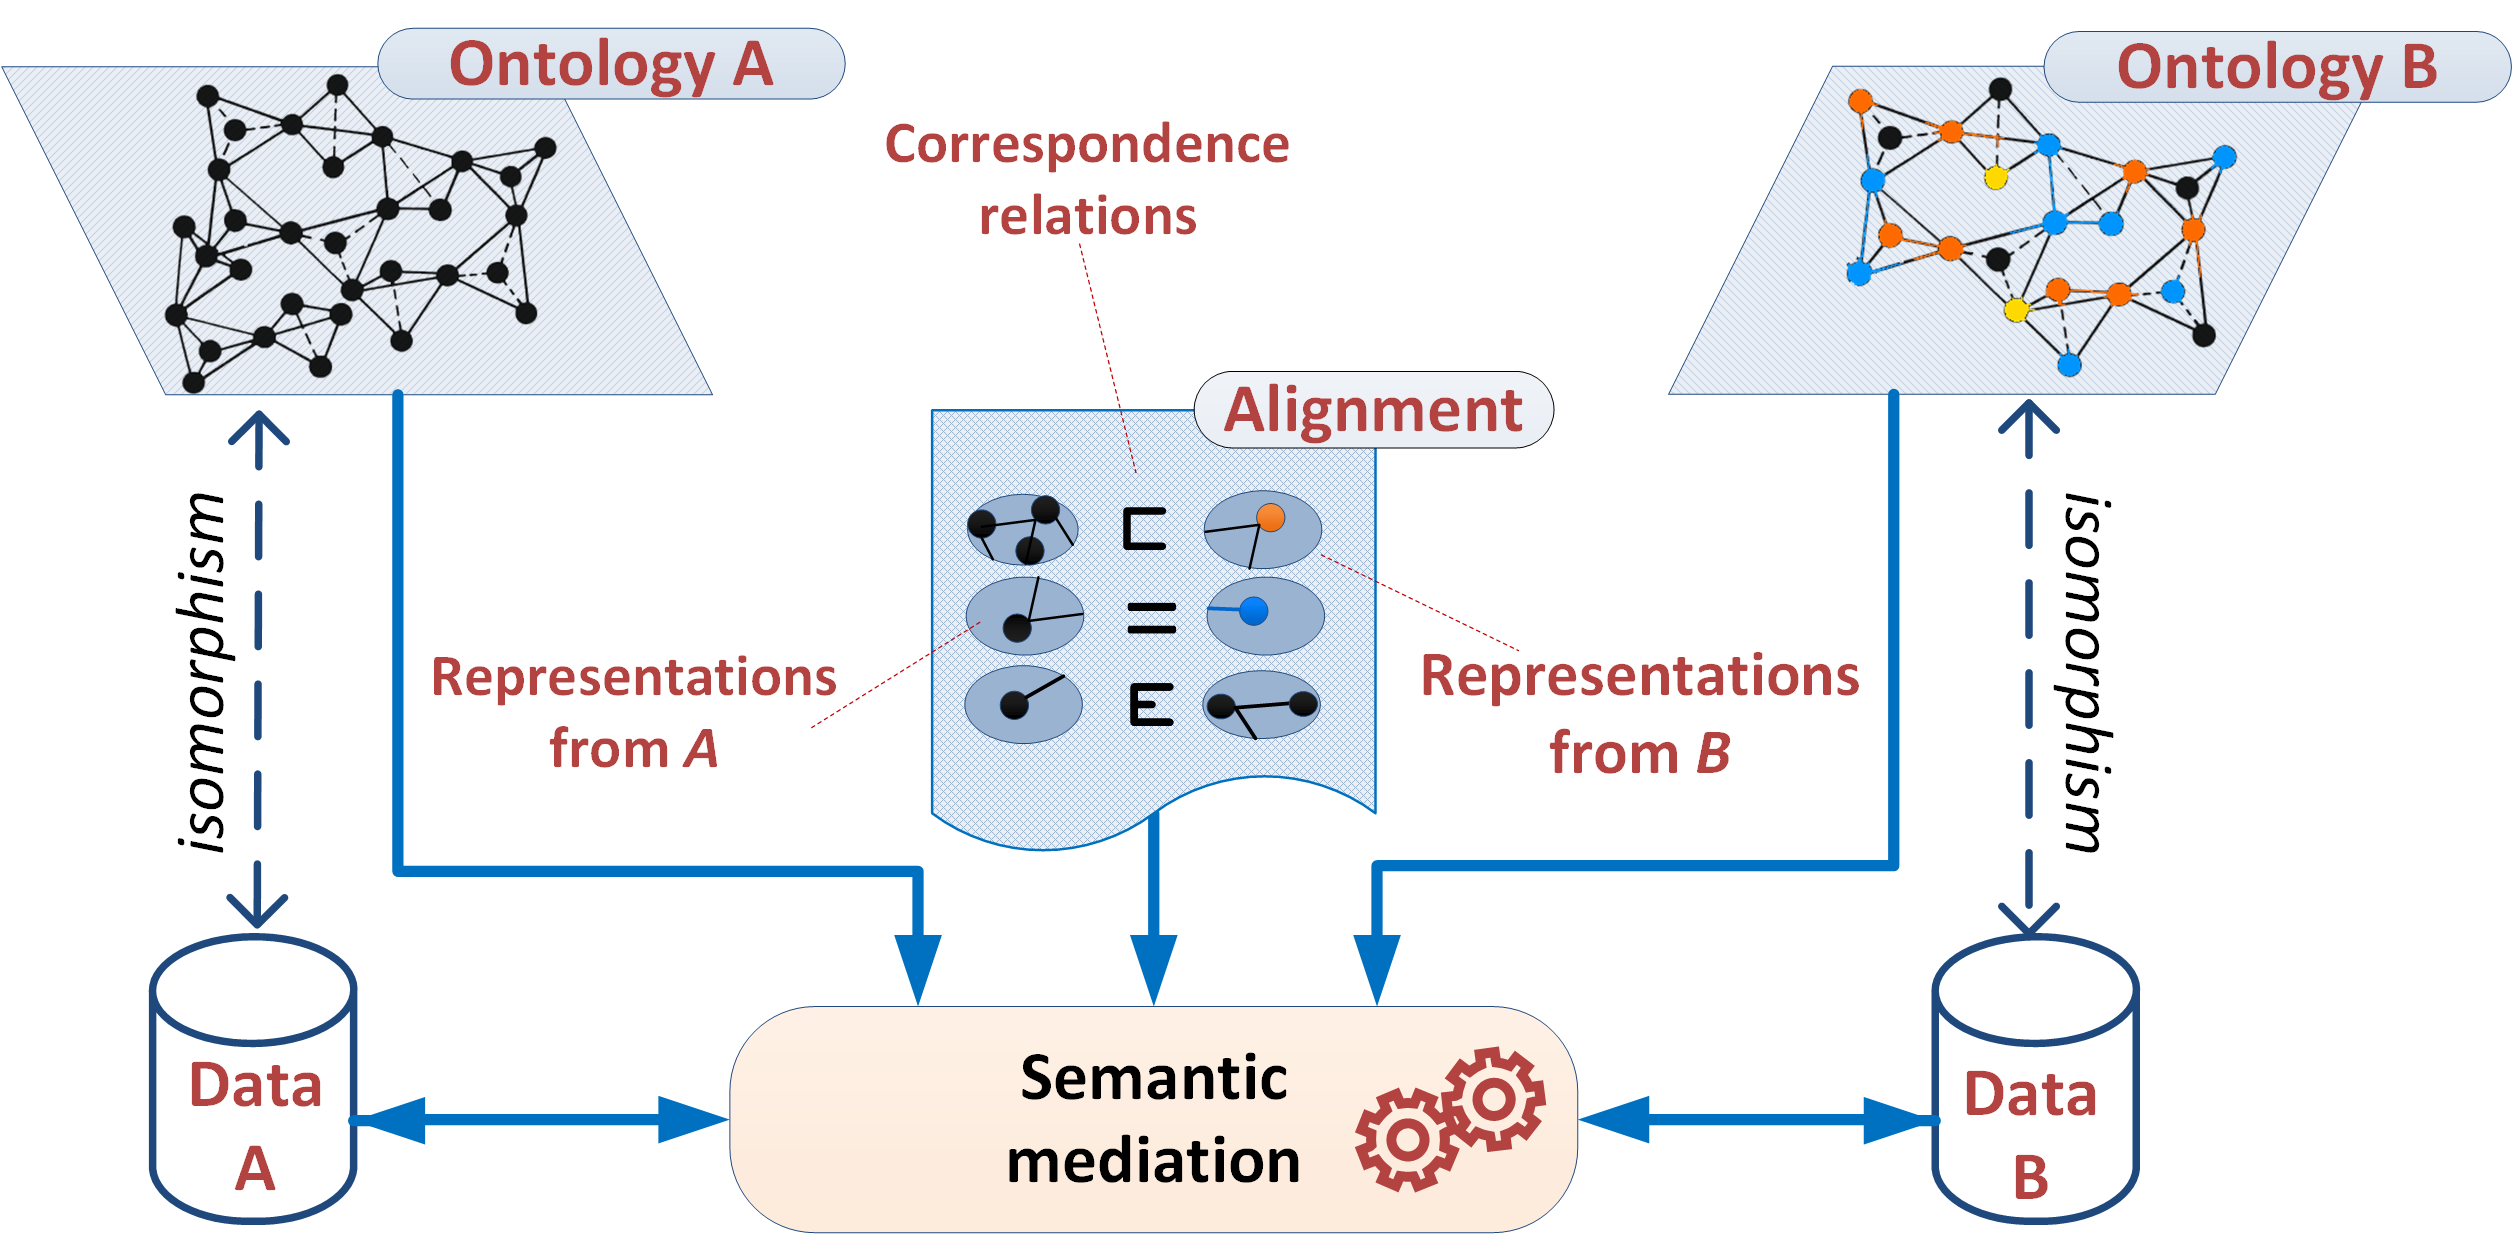
\includegraphics[width=0.75\textwidth,height=\textheight]{src/images/RunTimeMediation.png}
\caption{Semantic mediation encapsulates how agents exchange semantic
meaning. It implements a generic transcription service between the
particular representations of data between both agents. It depends only
on the representations of the semantic meaning from both agents
(ontologies) and the alignment that holds between
them.}\label{fig:rt-mediation}
}
\end{figure}

We have seen in the previous sections that a correspondence assures the
semantic validity between the different semantic meanings of both
agents. It can do so by token of the broad correspondence relations that
can be specified, both for the conceptual and the value differences that
may exist between them. Unfortunately, this is in shear contrast with
the fact that a transcription can only replace one term for another,
which basically implies that an equivalence relation holds between both
terms. As can be seen from the correspondence relation, this is not
necessarily true. In \citep{Brandt2018b}, we make a distinction between
a naive transcription, which ignores this inconsistency, and a semantic
valid transcription that can establish under what conditions this
inconsistency does not yield phantom semantics. We show that these
conditions rely on logical constructs only and, consequently, are
independent on the actual ontologies that apply. We have formulated
these logical constructs as rules that generically apply for any
transcription. Unfortunately, a set of conditions remain for which a
semantic valid transcription cannot be guaranteed, either due to an
incomplete alignment or to (onto)logical incorrect correspondences. It
follows that a semantic mediation service must provide for options about
the resolution for these remaining issues. We suggest at least the
following options: Firstly, as run-time options we consider (i) a means
to fall-back to the application of naive transcriptions and continue the
data exchange, or (ii) to raise a Transcription Error and refrain from
data exchange. Both represent necessary service implementations that
might satisfy scenarios that have either less or more stringent semantic
demands. Secondly, as design-time option, it serves as a necessary tool
to generate an exhaustive list of shortcomings of the transcription as a
result of the current ontologies and alignment. Such list will provide
the semantics engineer with sufficient information to adapt the
alignment, or introduce modifications to one or both of the semantic
anchorages in order to remove transcription issues that are considered
vital to the business. Finally, the third option is to try to resolve
the transcription issue by starting a dialogue-based semantic
reconciliation process in run-time with the aim to improve upon the
shortcomings of the current alignment. Despite our insistence on the
need for a human to author the genuine understanding, it might still be
worthwhile to have the system meticulously, consistently and
methodologically negotiate logical and ontological constructs in order
to find additional correspondences \citep{Diggelen:2007vd}.

\hypertarget{evaluation-of-siop-principles}{%
\section{Evaluation of sIOP
principles}\label{evaluation-of-siop-principles}}

The main (business) requirement is to achieve sIOP as quickly as
possible, with as minimal effort as possible, for collaborations that
had not been foreseen and consequently could not be anticipated for
during design time of the (two or more) software agents. We have
introduced some new principles to its support in the previous sections,
and now evaluate their consequences on the objectives as elaborated in
\cref{objectives-of-semantic-interoperability}, particularly those that
refer to the engineering challenges: two (loose coupling at semantic
level), three (allow for semantic heterogeneity), five (support to
semantic evolution) and six (scalable semantics).

\hypertarget{loosely-coupled-semantics}{%
\subsection{Loosely coupled semantics}\label{loosely-coupled-semantics}}

Consolidating sIOP demands the emergence of \emph{loosely coupled
semantics}. As analogy, consider a vehicle with its cargo. Logistics
rely on external transfer services that allow the cargo to be
transported over different vehicles, from a truck into an aircraft into
ship into a truck again, without ruining the cargo. This requires the
cargo to be firmly connected to the vehicle, but at the same time to be
completely independent from any particular vehicle in order to complete
the transport. ``Connected but as independent as possible'', also known
as loosely coupled, is a need for sIOP as well. When software agents
interact they exchange meaning. Loosely coupled semantics implies that
the semantic meaning (the cargo) remains as independent from the
representation of semantics (the vehicle) as possible. Similarly to
logistics, sIOP should rely on infrastructural services that can
transcribe the semantic representation from its native form into a
foreign form without invalidating the semantics that it bears. Loose
coupling is known as a strong characteristic which brings many
advantages. This applies to its semantic variety as well: agents can now
communicate in their own native representations without the need to
learn or integrate foreign representations; define semantics once and
achieve sIOP many times with many different peers; development of the
agents' semantic representations can be locally isolated to fit their
particular domain and application; and it enables local re-use which on
its turn increases its quality.

Loose coupling in the classical sense is realised through the principles
of separation of concerns and transparency. In its original reading
separation of concerns turns complex functionalities into simple, atomic
and complementary functional capabilities. In a semantic reading
separation of concerns is not about maintaining complementary semantics;
in fact, the domain of interest of the agents are required to overlap,
since interoperation would be completely useless otherwise. Instead,
semantic separation of concerns refer to enforce an explicit division
between syntax and semantics, as discussed in
\cref{explicit-siop-by-alignment}. Additionally, it refers to keeping
each other's representations of the semantic meaning strictly separated.
We described how this can be achieved in \cref{roadway-mediation}. The
classical results of applying the principle is the emergence of unique
functions that are implemented only once and used many times. In its
semantic application this results in every software agent to maintain
its own semantics. Collectively, all agents make that semantics become
distributed all over the place which seems counterintuitive or even
plain wrong. We come back to that intuition when we talk about
scalability, \cref{scalable-siop}, but we can already see that this is
an indirect consequence of the demand to enable sIOP with agents that
were not anticipated for during software design; this, on its turn,
requires that independent development of semantics shall be possible
without disabling sIOP.

The classical reading on transparency separates access to the unique
functions from the particular design and implementation of the
functions. Remaining agnostic to \emph{how} its function are achieved
makes it possible to communicate with minimal mutual dependency.
Semantic transparency, or terminology transparency, remains agnostic to
how semantics are \emph{represented}, which makes it possible to
communicate with minimal syntactic dependency and without prior mutual
agreements on semantic representation. In its classical reading,
transparency requires the introduction of standards in the components'
API. Semantic transparency, contradictory, requires the total absence of
any standard on representation. In stead, semantic transparency, too,
requires to separate semantics from syntax. Furthermore, a need emerges
for a semantic oracle that knows how to align distinct representations
and to translate between them accordingly. The latter has already been
discussed in \cref{roadway-mediation} while the former is directly
related to the human-in-the-loop as authoring authority as discussed in
\cref{spanning-semantic-interoperability}.

From the above discussion we draw the conclusion that all demands
necessary to allow for semantic separation of concerns and semantic
transparency are met by the sIOP principles
\cref{dp:ssoc,dp:alignment,dp:mediation}. Therefore, loosely coupled
semantics should emerge between agents that comply to these principles.

\hypertarget{semantic-heterogeneity-1}{%
\subsection{Semantic heterogeneity}\label{semantic-heterogeneity-1}}

We have already determined that the principle to align semantics as
opposed to data schemata, \cref{dp:ssoc}, breaks the conflation of
semantics and syntax, enabling to consider semantics on its own
terms\footnote{Pun not intended}. Abstaining from a canonical model by
introducing a semantic alignment between pairs of semantic meanings,
\cref{dp:alignment} introduces the capability for each agent to develop
its semantic representation in a way that fits its local perspective
optimally. By also encapsulating the particular means to provide valid
semantic transcriptions only and refrain from naive transcriptions
between communicating agents, \cref{dp:mediation}, the necessary
elements to support semantic heterogeneity are present.

\hypertarget{semantic-evolution}{%
\subsection{Semantic evolution}\label{semantic-evolution}}

Consider an agent who's local semantics are in demand for a change.
Assume that the agent has modified its internal pragmatic meaning to
accommodate the evolved semantics. This implies a change in what we
called the semantic anchorage, which acts as semantic interface to any
sIOP concerns. The semantic change can be considered an altered or
additional difference with the semantic anchorage from interoperating
peer agents. In order to not destroy the sIOP that had been established
before, it is necessary to reflect the new difference as modifications
to the alignments that apply. By having performed the necessary
modifications, and by relying on the semantic validity of the own
ontology, the mediator is now capable of transcribing the data in
accordance to the evolved semantics.

The consequence of allowing semantic heterogeneity is therefore a
sufficient condition to also enable local semantic evolution and
remaining semantic interoperable with existing counterparts in the
process.

\hypertarget{scalable-siop}{%
\subsection{Scalable sIOP}\label{scalable-siop}}

Many definitions exist to constrain the semantics of \emph{scalability},
academic \citep[e.g.,][]{Neuman1994} and popular\footnote{http://www.linfo.org/scalable.html,
  accessed Nov.~2019; https://en.wikipedia.org/wiki/Scalability,
  accessed Nov.~2019} alike. Our summary refers to increasing the demand
that is placed on a system, and/or adding resources to a system, without
experiencing loss of performance or increase in management to an extent
that defeats its primary objective. We consider scalable sIOP as the
capability to allow for increase in number of communicating agents as
well as in the level of semantic heterogeneity without degrading the
agent's communication performance or its ability to manage and control
the semantic differences with its interoperating peers.

If we consider the agent's communicating performance degradation, we
argue that since complexity of the connections have been traded with the
complexity in the mediator (\cref{roadway-mediation}), the agent will
only experience communication degradation when the mediator experiences
transcription latencies that exceed communication parameters. In other
words, the performance bottleneck is with the mediator, not with the
agent. Transcription latency will result from the number of
transcription requests that exceeds the capacity of a single mediator.
No particular mechanism in a mediator impedes horizontal scaling to
increase the collective processing capacity to match the transcription
demands.

Regarding the ability to manage and control the semantic differences
with all interoperating peers, the root cause for potential alignment
management issues are laid in the need to establish an alignment with
each peer agent an agent collaborates with. This might become
impractical due to our insistence on the need for a human-in-the-loop to
author the alignment. We discern different solutions for different
semantic topologies:

\begin{enumerate}
\def\labelenumi{\roman{enumi}.}
\tightlist
\item
  Star alignments (core domain ontology, aligned to local ontologies)
  for relative stable and homogeneous domain semantics

  \begin{itemize}
  \tightlist
  \item
    Good: semantic governance remains controllable independent from the
    number of actors;
  \item
    Bad: very big semantic monolith, hence, low agility in dynamic
    environments. Moreover, the more actors involved, the higher the
    need for semantic compromises, and the lower the overall semantic
    accuracy.
  \end{itemize}
\item
  Mesh alignments (bilateral alignments) for very dynamic and
  heterogeneous (domain) semantics, or low number of peers

  \begin{itemize}
  \tightlist
  \item
    Good: quickly established bilateral sIOP; granularity-on-demand, viz
    intricate where necessary, coarse-grained where possible;
  \item
    Bad: semantic governance may become an issue to the level where it
    becomes impractical.
  \end{itemize}
\item
  Mix-n-Match (coarse-grained star-alignment with intricate bilateral
  alignments as specialisations to the core domain ontology) for the
  70\% bulk

  \begin{itemize}
  \tightlist
  \item
    Good: controllable semantic governance; after central alignment,
    quickly established bilateral sIOP;
  \item
    Bad: slightly more complicated mediation due to double alignment
    support.
  \end{itemize}
\item
  Daisy-chained alignments (when A is aligned to B, and B is aligned to
  C, A and C are indirectly aligned as well)

  \begin{itemize}
  \tightlist
  \item
    Good: self-organised alignments emerge, and an instantaneous
    access-and-play becomes possible;
  \item
    Bad: No guarantees can be given on the completeness of the indirect
    alignment. Furthermore, more intermediate alignments will increase
    the chance of impossible end-to-end transcriptions that would not
    occur with a direct alignment.
  \end{itemize}
\end{enumerate}

In conclusion, scalable sIOP can be guaranteed when considering the
communication performance. With respect to the ability of a single agent
to manage and control the number of alignments with increasing number of
interoperating agents, several options exist to support scalable sIOP
although ultimately no guarantees can be given.

\hypertarget{iso42010-viewpoint-on-siop}{%
\section{ISO42010 viewpoint on sIOP}\label{iso42010-viewpoint-on-siop}}

\hypertarget{related-work}{%
\section{Related work}\label{related-work}}

Discuss the following papers:

\begin{enumerate}
\def\labelenumi{\arabic{enumi}.}
\item
  https://scholar.google.com/citations?user=pkJy5p8AAAAJ\&hl=en
\item
  Pahl, C. (2007). Semantic model-driven architecting of service-based
  software systems. Information and Software Technology, 49(8),
  838--850. https://doi.org/10.1016/J.INFSOF.2006.09.007
  ---\textgreater{} Compare how they apply onto's for DM
\item
  Maybe discuss as agreement-based approach to sIOP: J.A. Mykkänen, M.P.
  Tuomainen, An evaluation and selection framework for interoperability
  standards, Information and Software Technology, Volume 50, Issue 3,
  2008,Pages 176-197, ISSN 0950-5849,
  https://doi.org/10.1016/j.infsof.2006.12.001.
  (https://www.sciencedirect.com/science/article/pii/S0950584906001960)
\end{enumerate}

Several works exist that focus on logical foundations of sIOP in search
for automatic matching and merging of ontologies
\citep{Euzenat:2013ie, Benedikt2018a, Scharffe2014}, or for automatic
detection and reconciliation of semantic inconsistencies between
ontologies \citep{Fahad2012, Diggelen:2007vd}. These works lay at the
heart of ontology mediation, however, their embedding in the larger
software environment is not addressed or only assumed at best. At the
same time, several works exist that address the architectural
foundations related to information analyses and interoperability, both
in academic literature \citep{Karagiannis2006, Raghupathi2008} and in
industrial practices \citep{ObjectManagementGroupOMG2013}. Few
literature exists on on the combination of foundations for architectural
concerns and those for formal semantics, and these make use of
ontological foundations to specify the semantics of the capabilities and
resources of the architectural language as opposed to domain semantics
\citep{Naudet2010, Azevedo2015, Carvalho2016}.

The authors of \citep{Pagano2013a} present an abstract account of
interoperability issues, research challenges and fundamental factors
that apply in interoperability. In terms of these findings, our work can
be considered on-topic, relevant, and in alignment with their research
agenda. It distinguishes from theirs by addressing sIOP solutions to
part of their broader and more abstract view on interoperability.

In \citep{Horsch2020} the authors discuss the ongoing work on
establishing a European Virtual Marketplace Framework, into which
diverse platforms can be integrated. It addresses common challenges that
arise when marketplace-level domain ontologies are combined with a
top-level ontology like the European Materials and Modelling Ontology
(EMMO) by ontology alignment. A multi-tier system of ontologies is
established with the EMMO at the top and all others subsumed by it. The
authors show that with such a setup the top-level ontology is crucial in
the creation of the alignments between the (domain)ontologies that are
subsumed by it. At the one hand this shows support to our conclusion
that semantic compatibility can be considered foundational to semantic
interoperability. At the other hand their particular approach is a
centralised one that does not scale well in large distributed
environments due to its dependency on one single ontological commitment.
Moreover, the top-level ontology, here EMMO, necessarily conflates its
function as ontological commitment with a function to construct
alignments from. Although this is of great help to resolving the
(automated) ontology matching problem, it creates a semantic monolith
that extends to all communicating peers which, as we have seen in
\cref{introduction}, impedes not only access-and-play sIOP but semantic
scalability, evolvability, maintainability and other qualities as well.

The automatic tabular document exchange (DocEx) framework proposed by
\cite{Yang2017} divides semantic interoperability into two stages:
\emph{interpretation}, described as automatic unambiguous information
understanding, and \emph{employment}, understood as the capability to
automatically operate on the information according to the interpreted
semantics. The interpretation phase is dependent on a global vocabulary
that ``provides uniquely coded and unambiguous concepts across different
domains''. Essentially, this is a clear example of the \emph{semantic
standard fallacy} described by \cite{Janowicz:2013ui}: ``The successful
standardisation of protocols made us believe that we should also
standardise meaning on the Web. This is a fundamental misconception'',
particularly since it defies semantic heterogeneity and different but
equally legitimate perspectives on the same thing. The authors remind us
of three limitations of the ontology alignment approach; firstly, it
cannot guarantee complete semantic interoperability for situations where
terms are not aligned; secondly, creating alignments are time consuming;
thirdly, ontologies are often local and their point-to-point alignments
limits the semantic consistency on a more global scheme. While we do not
deny any of these we consider that (i) alignments exist to facilitate
interoperability, hence, lacuna are to be (automatically) corrected;
(ii) their creation, despite ontology matching algorithms and other
automation, will take time but allow for local semantic qualities and
independence that are impossible to achieve with a global semantic
standard; (iii) local applications are not seeking for global
interoperability but business network interoperability only.

The DocEx framework can be considered a simplified version of the
openEHR framework\footnote{https://www.openehr.org/, accessed Jan 24,
  2020} as introduced by \cite{Beale:2001vz}, further elaborated in
\citep{Beale2007a, Beale2008a, Beale2007, Beale2008, Beale2007b, Beale2007c}
and incorporated into CEN 13606 as a European and ISO standard. Its
founding key paradigm is to model generic knowledge apart from the
specific information structures, and let the former constrain the
latter: knowledge is expressed as ``statements which say how instances
of a reference model should be constrained to form a valid business
entity of some kind''. Those statements are embodied by
\emph{archetypes}. They introduce a Reference Model (RM) that can be
semantically constrained by an Archetype Model (AM). The latter can be
considered a meta-model or modelling language to express archetypes,
i.e., a particular semantic model representing knowledge. The former is
provided to each stakeholder as a unified software implementation (``the
run-time platform''), providing invariant patterns of information
structures. This separation makes what the RM is to the AM similar to
what the JVM is to the java program. Any information item created by a
user is registered as an instance of RM-specified invariant patterns. At
the same time that information item is conforming to an archetype that
expresses (constrains) its semantics in terms of the AM. Such approach
follow \cref{dp:rfsm,dp:meoc} but the application of a central
definition of archetypes maintain a tight coupling and thus defies
semantic heterogeneity and truly independent semantic representations.

The authors in \citep{Haller2005} propose the Web Service Execution
Environment (WSMX) that enables the execution of Semantic Web Services
based on a Web Service Modelling Ontology (WSMO), and consider it a
reference implementation for WSMO. It is meant as a means for automated
discovery, composition and execution of Web Services which are based on
logical inference-mechanisms, and in this way similar to our objective.
Another similarity is in their acceptance of semantic heterogeneity and
the need for a generic data mediator to overcome semantic differences,
thereby following \cref{dp:ssoc}. Despite these similarities, we
consider two main differences with our approach. Firstly, the goals of
WSMO are of another, broader, dimension than our goal to consolidate
semantic interoperability and for which we have introduced details that
are out of scope of WSMO. \textbf{\emph{Secondly,}}

Recently the international data spaces (IDS) association\footnote{https://www.internationaldataspaces.org/the-principles/\#overview,
  accessed Jan 28, 2020} forms the basis for a data marketplace as a
strategic link between the creation of data in the internet of things
and applying this data in machine learning (ML) and artificial
intelligence (AI) algorithms. The proposed architecture,
\citep{Otto2019}, is much alike the WSMX in the sense that a
well-defined connector provides infrastructural services concerning
security and trust, sovereignty, interoperability, ease of adoption and
use, and more. In fact, if we conceive WSMX as an abstracted version of
Web Services with a particular attention to semantics, IDS can be
conceived as an abstracted version of the REST framework that considers
data resources (spaces) the central assets in an ecosystem. IDS puts a
particular attention to technology transparency when it comes to asset
discovery and disclosure, identity, their secure, managed and
accountable use, and interoperability. IDS considers data as assets, and
provides many if not all necessary components for its managed exchange.
Contrarily, we observe a clear absence of any considerations similar to
those we bring forward in this paper towards the consolidation of sIOP.
Still, and like WSMX's and our objectives, IDS clearly intends to put
forward an architectural design with the aim to solve the concerns
generically into a transparent infrastructure. In conclusions, we
consider IDS' data technology transparency an interesting complement to
our data semantic transparency.

\citep{Greefhorst2011} provides for a Principles Catalogue in their
appendix which presents almost sixty design principles. Principle A.20
of them reads \emph{Data that are exchanged adhere to a canonical data
model}, and one of its rationals states that \emph{A Canonical Data
Model standardises the definitions of data that are exchanged (\ldots)}.
Indeed, principle A.20 reflects the current practises to achieve
interoperability. Although it conflicts with \cref{dp:ssoc}, it is not
necessarily wrong, since following it results in achieving
interoperability as justified by the many if not all interoperable
systems that exist today. However, its application impedes
access-and-play interoperability as well as semantic heterogeneity, as
we have shown in \cref{waar-precies}.

In support of EU's single digital market, the new European
Interoperability Framework (EIF) \citep{EU-ISA2Program2019} gives
guidance to public administrations on how to improve interoperability.
It provides three recommendations on the semantic level which are rather
abstract in their formulation, although exemplifying these with
approaches that can be categorised in FEI \citep{Chen2017} as
\emph{integrated}, or \emph{unified} at best, but not \emph{federated}.
These examples imply that our approach is not in compliance with the
EIF, which is in contrast with the three recommendations that do not
exclude a \emph{federated} approach, or any other of the DPs that we
have elaborated.

The authors of \citep{Neiva2016} present a literature research to
pragmatic interoperability. Although no definition on pragmatics or its
interoperability is given, the distinction with semantics is given as
``semantics is related with which the {[}semiotic{]} sign refers to, and
pragmatics is related to the effect of the sign on the interpreter.''.
This aligns with our application of semantic meaning and pragmatic
meaning. Where the authors keep pragmatics separate from semantics and,
therefore, treat pragmatic interoperability separate from semantic
interoperability, we consider the reciprocity between them significant
and conclude that semantic interoperability can only be achieved when
the DSC can re-establish the connection of the DSP's data with its own
pragmatic meaning. Opposed to the authors opinion, we consider the
pragmatic meaning a necessary element in achieving sIOP.

A quasi-systematic literature review to interoperability in
context-aware software systems was undertaken by \citep{Motta2019},
resulting in an Interoperability Theoretical Framework ``used to guide
the evolution of software systems regarding changes focused on
interoperability''. They identify 16 high-level interoperability
mechanisms, i.e., decisions to be taken and solutions recurrently used
throughout the software systems to achieve interoperability. Our design
principles are in (partial) support of 12(3) of the mechanisms, i.e.,
``Use common ontologies to enable understanding'', and ``Use `bridges'
to enable interaction''. The 4 mechanisms that we do not support can be
considered out of our scope, e.g., ``Use opens source solutions'' or
``Use suitable protocols''.

\hypertarget{discussion-future-work}{%
\section{Discussion \& future work}\label{discussion-future-work}}

Complement weak AI with human brain:

\begin{itemize}
\tightlist
\item
  use AI where possible (computational semantics for software agent;
  supporting semantic reconciliation)
\item
  use human brain where necessary (but not more): ontology engineering @
  design time; alignment authoring @ pre-runtime

  \begin{itemize}
  \tightlist
  \item
    Therefore, and no matter how the human will be positioned in the
    architecture, in its pure sense, an access-and-play capability can
    never be established. However, the time-to-deliver sIOP between two
    interoperating software agents can be dramatically reduced.
  \end{itemize}
\end{itemize}

\onecolumn

Throughout this document, the following Design Principles have been defined. 

%%%%%%%%
%%
%% Tex code representing Design Principles Table
%%
\def\arraystretch{0} 
\begin{xltabular}[l]{\linewidth}{@{} >{\small\raggedright\arraybackslash}p{0.47\linewidth} >{\small\raggedright\arraybackslash}X @{}}

\caption{The sIOP design principles; structured according to \cite{Greefhorst2011} \label{tab:dps}} \\
\toprule
\multicolumn{1}{@{}l}{Design Principle} & \multicolumn{1}{l}{Dimensions \& Attributes} \\ 
\multicolumn{1}{l}{Rationale} & \multicolumn{1}{l}{\quad Implications} \\ \cmidrule(r){1-1} \cmidrule(l){2-2}
\endfirsthead
\multicolumn{2}{@{}l}{\ldots\ \tiny Continuation}\\ \midrule
\multicolumn{1}{@{}l}{Design Principle} & \multicolumn{1}{l}{Dimensions \& Attributes} \\ 
\multicolumn{1}{l}{Rationale} & \multicolumn{1}{l}{\quad Implications} \\ \cmidrule(r){1-1} \cmidrule(l){2-2}
\endhead
\midrule\multicolumn{2}{r@{}}{\tiny Continued \ldots}\\
\endfoot
\endlastfoot
%
%
%
%%%%%%%%%%%%%
%%
%% SEMANTIC HETEROGENEITY PRINCIPLE
%%
\begin{mmdp}\label{dp:shp}{\bfseries Semantic heterogeneity principle:}
\quad sIOP should strive to support multiple co-existing perspectives of use as opposed to enforcing one single perspective, and should be founded on the active reconciliation of semantic differences rather than on allowing one homogeneous semantic standard only.
\end{mmdp}
&
\begin{description}[labelwidth=3.7cm,leftmargin=3.7cm+1ex,nosep,topsep=2ex,labelsep=1ex,font=\bfseries]
  \item[Type of information:] business, data  
  \item[Quality attributes:] semantics, interoperability, reliability, reusability, efficiency
\end{description} \\
\begin{enumerate}[left=6pt, nosep]
  \item The user of the software agent has a natural, business-controlled perspective on the DoA;
  \item Data represent the state of affairs about that DoA, viewed from a particular perspective of use;
  \item Semantics of data, and with it the faithfulness with which the data refers to reality, is directly dependent on the perspective of use;
  \item Such view is just one particular perspective out of many equally legitimate ones;
  \item Equally legitimate perspectives on reality naturally create semantic heterogeneity;
  \item Accepting semantic heterogeneity implies the probable uniqueness of the agents view on reality;
  \item Without adherence to this principle, sIOP can be achieved only for dedicated DSC/DSP pairs, with collaborations that have been foreseen, for which the semantics are assumed stable over time, implemented with technology or platforms for which no or limited evolution is anticipated, and assuming that new collaborations won't emerge over time.
\end{enumerate}
&
\begin{enumerate}[left=10pt, nosep]
  \item Semantic heterogeneity allows software agents to maximise their semantic clarity, accuracy and, consequently, the faithfulness of its representation of the SoA in its DoA;
  \item Semantic heterogeneity allows software agents to be developed independently from each other, and particularly from potentially collaborative software agents;
  \item Semantic heterogeneity weakens the need to coordinate semantic specifications centrally; in stead, “anyone can say anything about any topic”, resulting in formalising the current state that semantic definitions are highly distributed;
  \item Maintenance and evolution of its semantics remain under the DSP’s own control throughout the whole lifespan of the agent, and only depends on its business interest for investment, no matter the growth and evolution of the domain;
  \item Semantic heterogeneity demands availability of semantic scalability solutions;
  \item Accepting semantic heterogeneity implies acceptance of semantic mediation and resulting semantic alignments in order to achieve sIOP.
\end{enumerate} \\
%
%
%
%%%%%%%%%%%%%
%%
%% SEMANTIC RESPONSIBILITY PRINCIPLE
%%
\begin{mmdp}\label{dp:srp}{\bfseries Semantic responsibility principle:}
\quad When it is reasonable to expect that the software agent will be engaged in collaboration or otherwise will interoperate with (an)other software agent(s), it is the responsibility of the DSP to disclose the semantic model of its DM and the ontological commitment that it applies, to the extent necessary for comprehension by the DSC.
\end{mmdp}
&
\begin{description}[labelwidth=3.7cm,leftmargin=3.7cm+1ex,nosep,topsep=2ex,labelsep=1ex,font=\bfseries]
  \item[Type of information:] Business, Data;
  \item[Quality attributes:] Semantics, interoperability, usability, efficiency;
\end{description} \\
\begin{enumerate}[left=6pt, nosep]
  \item Assume semantic heterogeneity to apply, resulting for the software agent in a particular perspective on the DoA;
  \item The semantic model mirrors the particular perspective taken, and applies a modelling language that expresses a particular OC that fits the perspective best; 
  \item Data are formulated according to the particular semantic model, and refer by means of it, to the SoAs in the DoA;
  \item Grice’s maxims on communication, and particularly on serving the quantity and manner of communication, represent the natural constraints to respect. Consequently, the responsibility to disclose the semantic model about the exchanged data, including its applied ontological commitment, can only lay by the DSP;
  \item Without adherence to this principle, the meaning of the data expressed by the software agent can be considered flawed, inaccurate, incomplete, even unavailable or otherwise insufficient in its support for semantic interoperability.
\end{enumerate}
&
\begin{enumerate}[left=10pt, nosep]
  \item The semantic model, which provides the semantic meaning to the data, is only dependent on the agent's own perspective on the application domain, and can therefore be designed independently from any other software agents;
  \item No matter the number of different communication peers, the software agent needs to specify the semantics of its data elements only once;
  \item By developing an explicit semantic specification of the data in advance, a software agent is prepared to engage in sIOP with other agents that can now connect to its semantics;
  \item By establishing collaboration with other DSPs or DSCs through its semantic model, the software agent ensures that the communication remains grounded in its own perspective.
\end{enumerate} \\
%
%
%
%%%%%%%%%%%%%%
%%
%% MINIMISE FAP PRINCIPLE
%%
\begin{mmdp}\label{dp:mfapp}{\bfseries Minimise FAP principle:}
\quad When it is reasonable to expect that the software agent will be engaged in collaboration or otherwise will interoperate with (an)other software agent(s), in order to minimise the False-Agreement Problem, its semantic model must be constrained to minimize the difference between the semantic meaning that it allows and those that is intended.
\end{mmdp}
&
\begin{description}[labelwidth=3.7cm,leftmargin=3.7cm+1ex,nosep,topsep=2ex,labelsep=1ex,font=\bfseries]
  \item[Type of information:] Business;
  \item[Quality attributes:] Semantics, interoperability, maturity;
\end{description} \\
\begin{enumerate}[left=6pt, nosep]
  \item The quintessential of exchanging data about the overlapping DoA is to indirectly exchange the SoA that the data refer to;
  \item Following \cite{Grice:1991BT}, it testifies to the quality of communication to take measures to prevent the exchange of SoAs that are invalid;
  \item The meaning that the agent's conceptualisation intends to convey is represented by a semantic model. Such representation can only approximate the intended meaning. 
  \item Therefore, the SoAs that are allowed by the semantic model do not necessarily represent the meaning that are intended by the conceptualisation. The difference between the allowed and intended meaning equals invalid meaning;
  \item Therefore, the agent should minimize the difference between the intended and the allowed meaning.
\end{enumerate}
&
\begin{enumerate}[left=10pt, nosep]
  \item When the allowed meaning of the semantic model encompasses the intended meaning as close as possible:
  \begin{enumerate}
    \item the DSP allows minimal room to convey invalid semantic meaning;
    \item the DSC allows minimal room to interpret the exchanged SoA invalidly;
  \end{enumerate}
  \item An overlap between the DSP's and DSC's semantic models then also implies a maximal overlap in what is intended to convey with a minimal overlap of invalid meaning; 
  \item The false agreement problem is reduced to the minimal extent possible;
  \item Note that this applies for interoperability between agents as well as re-usability of the DM by other agents;
\end{enumerate} \\
%
%
%
%%%%%%%%%%%%%%
%%
%% SEMANTIC PROTOCOL PRINCIPLE
%%
\begin{mmdp}\label{dp:spp}{\bfseries Semantic protocol principle:}
\quad When it is reasonable to expect that the software agent will be engaged in collaboration or otherwise will interoperate with (an)other software agent(s), the agent should provide the capability to respond to a semantic protocol that has the objective to prepare sIOP by conversing about semantics in order to consolidate semantic compatibility and mutual comprehension of the exchanged data.
\end{mmdp}
&
\begin{description}[labelwidth=3.7cm,leftmargin=3.7cm+1ex,nosep,topsep=2ex,labelsep=1ex,font=\bfseries]
  \item[Type of information:] Business;
  \item[Quality attributes:] Semantics, interoperability, efficiency;
\end{description} \\
\begin{enumerate}[left=6pt, nosep]
  \item Following \cite{Grice:1991BT}, it testifies to the relation of communication to clarify the purpose of the communication;
  \item The essence of sIOP is to exchange SoAs about the DoA;
  \item Before SoAs can be exchanged, sIOP must be prepared by establishing agreement on the data's semantic meaning, the semantic models used, achieving semantic compatibility and the semantic topology that applies;
  \item This implies to recognise the purpose and subject of communication, and hence, to maintain a shared vocabulary and communication process to denote them and switch between them, viz to rely on a standard semantic protocol.
\end{enumerate}
&
\begin{enumerate}[left=10pt, nosep]
  \item A semantic protocol can be considered a bootstrapping process, from establishing agreement on what protocol and version to use (if more than one is available), to being ready to engage in exchanging SoAs;
  \item A semantic protocol talks about semantic meaning and can therefore be considered to operate on a meta-semantic level, implying that it is independent from the particular semantics that apply to the exchanged SoA;
  \item This allows the semantic protocol to become an infrastructural service in support of sIOP.
\end{enumerate} \\
%
%
%
%%%%%%%%%%%%%
%%
%% ALIGNMENT PRINCIPLE
%%
\begin{mmdp}\label{dp:alignment}{\bfseries Alignment principle:}
\quad Aligning semantic meanings suffices for re-establishing semantic coherence and, hence, enabling sIOP. \end{mmdp}
&
\begin{description}[labelwidth=3.7cm,leftmargin=3.7cm+1ex,nosep,topsep=2ex,labelsep=1ex,font=\bfseries]
  \item[Type of information:] Application, Data;
  \item[Quality attributes:] Semantics, semantic interoperability;
\end{description}\\
\begin{enumerate}[left=6pt, nosep]
  \item On processing (external) data, semantics manifest themselves as the reciprocity between semantic meaning (carried by data) and pragmatic meaning (carried by processing code);
  \item The purpose of an alignment is to re-establish semantic coherence between the DSP's semantic meaning and the DSC's pragmatic meaning, as specified by the DMs of the software agents;
  \item Formalising a correspondence relation between the semantic meanings of interoperating software agents effectively connects the external semantic meaning with the internal pragmatic meaning, providing the existence of semantic coherence by the DSC;
  \item By assuring that the internal semantic meaning encompasses the external semantic meaning, and by assuring that the semantic consequences of the latter extending the former are (or can be made) insignificant for the available semantic coherence, consolidates the semantic validity of the correspondence relation.
\end{enumerate}
&
\begin{enumerate}[left=10pt, nosep]
  \item The conversion from external to internal semantic meaning is specified by a correspondence;
  \item The collection of all correspondences specify the semantic alignment that holds between a pair of interoperating agents;
  \item Software agents that are unable to align their semantic meaning with the external semantic meaning cannot engage in sIOP without introducing phantom semantics, with unforeseen consequences in their data processing;
  \item Despite the assumption that computers are token-based only without the capability to establish semantics, authoring the semantic alignment necessarily remains the \emph{only} human effort in establishing sIOP.
\end{enumerate} \\
%
%
%
%%%%%%%%%%%%%
%%
%% CORRESPONDENCE RELATION PRINCIPLE
%%
\begin{mmdp}\label{dp:alignment-language}{\bfseries Correspondence relation principle:}
\quad A correspondence relation that preserves semantic meaning addresses conceptual differences as well as convention-induced value space differences, the resolution of which is a necessary condition to achieve sIOP (providing faithful DMs from both collaborating agents). \end{mmdp}
&
\begin{description}[labelwidth=3.7cm,leftmargin=3.7cm+1ex,nosep,topsep=2ex,labelsep=1ex,font=\bfseries]
  \item[Type of information:] Data;
  \item[Quality attributes:] Semantics, semantic interoperability;
\end{description}\\
\begin{enumerate}[left=6pt, nosep]
  \item Assume the DSP and DSC each have their semantics faithfully specified by domain models;
  \item Assume that the DMs of the DSP and the DSC are compatible but express differences in their conceptualisation underlying their semantic meaning, resulting from alternate perspectives on the DoA;
  \item Then, assume we ignore:
  \begin{enumerate}
    \item the preservation of semantic meaning: then the DSC is allowed to ultimately refer to different individuals and, hence, a different SoA than specified by the DSP; 
    \item meta-properties of the relation between the concepts: then the DSC is allowed to infer SoAs that are not warranted by its premises;
    \item constraints to falsify possible interpretations: then the DSC allows SoA that are not intended by the DSP; 
    \item units of measurement: then the DSC allows the Mars Climate Orbiter to crash into the Martian atmosphere \cite{Leveson2004};
    \item lower value scale resolution: then the value masks distinctions that the DSC can comprehend as a different SoA than it will act upon;
    \item distinctions between ordinal, interval and ratio scales: then the DSC is allowed to make comparisons between incomparable values, resulting in invalid pragmatic meaning;
  \end{enumerate}
  \item Without addressing the conceptual and (convention-induced) value space differences, sIOP cannot emerge.
\end{enumerate}
&
\begin{enumerate}[left=10pt, nosep]
  \item With the exception of value space differences that originate from measurement system characteristics, convention-induced value space differences and conceptual differences can be specified such that preservation of semantic meaning can be guaranteed;
  \item Although correspondence relations are to be specified for each and every difference that applies in semantic meaning between the DSP and DSC, the modeling language to represent alignments remains agnostic to the specifics of the DMs involved (except for the representation of individuals in the DM).
\end{enumerate} \\
%
%
%
%%%%%%%%%%%%%
%%
%% SEMANTIC SEPARATION OF CONCERNS PRINCIPLE
%%
\begin{mmdp}\label{dp:ssoc}{\bfseries Semantic separation of concerns principle:}
\quad When a software agent engages in interoperation with (an)other software agent(s), separate data communication services from data comprehension and business collaboration services, and, separate the domain model in areas that show high cohesion and low coupling. \end{mmdp}
&
\begin{description}[labelwidth=3.7cm,leftmargin=3.7cm+1ex,nosep,topsep=2ex,labelsep=1ex,font=\bfseries]
\item[Type of information:] Data, Technology;
\item[Quality attributes:] semantic interoperability, portability, maintainability, efficiency, usability (reuse), reliability, functionality;
\end{description}
\\
\begin{enumerate}[left=6pt, nosep]
  \item Data schemata are defined to support the (de)serialisation processes that consolidate the data communications concern;
  \item Neglecting the principle of separation of concerns solidifies dependency between otherwise disjoint concerns, here the semantic level and the syntactic level of data communication;
  \item Access-and-play capabilities are supported by assuring minimal impact on software code when introducing semantic modifications;
  \item Minimising impact on software code that is concerned with data communication is realised by abstracting semantics away from the data schemata;
  \item When the DM defines a high variety of subjects in the DoA without a clear separation between them, a small change in semantics will induce a proliferation of modifications in the DM;
  \item Modularisation of the DM minimises the proliferation of a change in one module to other modules.
\end{enumerate}
&
\begin{enumerate}[left=10pt, nosep]
  \item Separation of concerns has a strong positive effect on software quality, including but not limited to sIOP;
  \item Removing any dependency between semantics and data syntax enables to support multiple communication paradigms without the need to modify the semantic representation;
  \item Similarly, modifications in the semantic representation, or supporting multiple semantic representations become possible without the need to modify the communication layer;
  \item SoC allows to align semantics as opposed to data schemata resulting the semantic reconciliation to be applied at a higher conceptual level, abstracting away from data communication schemata;
  \item Heterogeneous semantics from multiple data sources are more easily supported;
  \item Semantic alignments imply the need for a mediation capability between the semantic representations of the communicating agents.
\end{enumerate} \\
%
%
%
%%%%%%%%%%%%%
%%
%% SEMANTIC TRANSPARENCY PRINCIPLE
%%
\begin{mmdp}\label{dp:st}{\bfseries Semantic transparency principle:}
\quad Remain agnostic to the local conceptualisation(s) and representation(s) of the agent(s) you collaborate with. \end{mmdp}
&
\begin{description}[labelwidth=3.7cm,leftmargin=3.7cm+1ex,nosep,topsep=2ex,labelsep=1ex,font=\bfseries]
\item[Type of information:] Data, Technology;
\item[Quality attributes:] semantic interoperability, portability, maintainability, efficiency, usability (reuse), reliability;
\end{description}
\\
\begin{enumerate}[left=6pt, nosep]
  \item Semantic heterogeneity is a matter of fact, and implies agents to apply different representations and conceptualisations on the DoA;
  \item For scalable sIOP to emerge these differences must be reconciled without introducing interdependencies between the DM's of the DSP and DSC;
  \item Remaining agnostic to local representations allows for sIOP without syntactic dependency;
  \item Remaining agnostic to local conceptualisations allows for sIOP without dependency on local semantic principles;
  \item Semantic differences, particularly about representation and conceptualisation, can then be resolved declaratively, defined only once for each DSP/DSC pair.
\end{enumerate}
&
\begin{enumerate}[left=10pt, nosep]
  \item Communicate without syntactic or conceptual dependency, in your own local representations founded on your own local conceptualisation;
  \item Governance and maintenance on semantics remain under one's own control;
  \item sIOP is realised declaratively, improving consistency of semantics, and allowing infrastructural components for generic semantic services;
  \item Semantic transparency enforces these semantic services, both infrastructural and agent-specific, to be \emph{about} semantics, demanding standardisation on the level of meta-semantics only.
\end{enumerate} \\
%
%
%
%%%%%%%%%%%%%
%%
%% SEMANTIC PROFILES PRINCIPLE
%%
\begin{mmdp}\label{dp:sprof}{\bfseries Semantic profiles principle:}
\quad Apply different semantic profiles for different collaborations. \end{mmdp}
&
\begin{description}[labelwidth=3.7cm,leftmargin=3.7cm+1ex,nosep,topsep=2ex,labelsep=1ex,font=\bfseries]
\item[Type of information:] Data, Technology;
\item[Quality attributes:] semantic interoperability, portability, maintainability, efficiency, usability (reuse), reliability;
\end{description}
\\
\begin{enumerate}[left=6pt, nosep]
  \item ;
  \item ;
  \item .
\end{enumerate}
&
\begin{enumerate}[left=10pt, nosep]
  \item ;
  \item ;
  \item ;
  \item .
\end{enumerate} \\
%
%
%
%%%%%%%%%%%%%
%%
%% SEMANTIC MEDIATION PRINCIPLE
%%
\begin{mmdp}\label{dp:mediation}{\bfseries Semantic mediation principle:}
\quad When software agents engage in interoperation, encapsulate the transcription between their semantic meaning.\end{mmdp}
&
\begin{description}[labelwidth=3.7cm,leftmargin=3.7cm+1ex,nosep,topsep=2ex,labelsep=1ex,font=\bfseries]
\item[Type of information:] Business, Data;
\item[Quality attributes:] Semantic interoperability, Consistency, reusability;
\end{description} \\
\begin{enumerate}[left=6pt, nosep]
  \item The semantic meaning is codified in ontological representations;
  \item Keeping agents from referring to each others representation therefore requires transcription between representations;
  \item A solution where each agent needs to implement one transcription component between its own representation and each of its interoperating peer, increases complexity;
  \item Encapsulating the transcription into an alignment-based intermediary component results in less communication complexity and relieves the agents from development and maintenance of local wrappers;
\end{enumerate}
&
\begin{enumerate}[left=10pt, nosep]
  \item A mediator creates representational transparency between communicating agents, keeping agents from using each others representations;
  \item This enables independent development of the individual agent’s semantic meaning;
  \item The need to enforce a canonical semantic representation, viz. semantic homogeneity, expires, allowing semantic heterogeneity to become the norm;
  \item Each agent can reuse its semantic anchorage in any other interoperation;;
  \item Transcription of the semantic meaning from the DSP representation and value space into the DSC representation and value space is only dependent on the applied alignment language and agnostic to any particular semantics assigned to it. A mediation component to perform such transcription, therefore, remains generically applicable for all domains. This provides the potential to turn the mediation component and the alignment language into infrastructural elements;
  \item Each agent can communicate with any other agent in its own native semantic representation.
\end{enumerate}\\
%
\bottomrule
\end{xltabular}
%%
%% END Design Principles Table
%%
%%%%%%%%%%%%%

\twocolumn

%%%%%%%%%%%%% APPENDICES
%% !ToDo!: Implement appendices.
%%
%% The Appendices part is started with the command \appendix;
%% appendix sections are then done as normal sections, i.e.,
%% \appendix
%% \section{}
%% \label{}

%%%%%%%%%%%%% ACKNOWLEDGMENTS
\section*{Acknowledgments}
P.B. would like to acknowledge Hanneke Dominicus for her editorial
efforts


%%%%%%%%%%%%% BIBLIOGRAPHY
%% If you have bibdatabase file and want bibtex to generate the
%% bibitems:
%% 1. Set the `bibliography` parameter in the pandocomatic configuration;
%% 2. Respect the related remarks from pandocomatic-elsarticle.template.
%%
\bibliography{src/bib/CitedByMe-2021-archSIOp.bib}
%%


\end{document}

%%
%% Note 1: For some reason that I cannot diagnose, the package `stackengine`
%%         is required with the `\longtable` command as it is being used in 
%%         elsarticle.latex; without its inclusion, the following error is
%%         thrown, referring to the first four lines after `\longtable`:
%% ! Undefined control sequence.
%% <argument> (\columnwidth - 6\tabcolsep ) * \real 
%%                                                  {0.2893}
%%         Anyone who can diagnose the source of this error, please inform me.
%%
%% End of file `elsarticle.latex'.
